\documentclass[11pt]{article}

\usepackage{comment} % enables the use of multi-line comments (\ifx \fi) 
\usepackage[a4paper,margin=1cm]{geometry}
\usepackage[utf8]{inputenc}
\usepackage[ngerman]{isodate}
\usepackage{gensymb}
\usepackage{graphicx}
\usepackage{booktabs}% http://ctan.org/pkg/booktabs
\usepackage{tabularx}
\usepackage{ltablex} % Longtables with tabularx
\usepackage[x11names]{xcolor}
\usepackage{amsmath}
\usepackage{amssymb}
\usepackage{amsthm}
\usepackage{array}
\usepackage{wrapfig}
\usepackage{subcaption}
\usepackage{csquotes}
\usepackage{lscape}
\usepackage{geometry}
\usepackage{multicol}
\usepackage{bm}
\usepackage{enumitem}
\usepackage{hyperref}
\usepackage{mdframed}
\usepackage{scalerel}
\usepackage{stackengine}
\usepackage{mathtools}
\usepackage{pdfpages}

% Code highlighting
\usepackage{minted}
\surroundwithmdframed{minted}

% Be able to caption equations and float them in place
\usepackage{float}

\newmdtheoremenv{theorem}{Theorem}

\theoremstyle{definition}
\newmdtheoremenv{definition}{Definition}[section]


\geometry{a4paper, margin=2.4cm}

\newcommand\equalhat{\mathrel{\stackon[1.5pt]{=}{\stretchto{\scalerel*[\widthof{=}]{\wedge}{\rule{1ex}{3ex}}}{0.5ex}}}}
\newcommand\defeq{\mathrel{\overset{\makebox[0pt]{\mbox{\normalfont\tiny def}}}{=}}}
\newcolumntype{C}{>{\centering\arraybackslash}X}

\newcommand*\samplemean[1]{\overline{#1}}
\newcommand*\ev[1]{\mathrel{\text{E}\left[#1\right]}}
\newcommand*\R{\mathbb{R}}
\newcommand*\Z{\mathbb{Z}}
\newcommand*\N[1]{\mathcal{N}\left(#1\right)}
\newcommand*\Likelihood{\mathcal{L}}
\newcommand*\diff{\mathop{}\!\mathrm{d}}
\newcommand*\Diff[1]{\mathop{}\!\mathrm{d^#1}}
\newcommand*\Exp[1]{\mathop{\text{Exp}}\left(#1\right)}
\newcommand*\Cov[1]{\mathop{\text{Cov}}\left(#1\right)}
\newcommand*\Cor[1]{\mathop{\text{Cor}}\left(#1\right)}
\newcommand*\Var[1]{\mathop{\text{Var}}\left(#1\right)}
\newcommand*\se[1]{\mathop{\text{se}}\left(#1\right)}


\DeclarePairedDelimiter\abs{\lvert}{\rvert}
\DeclarePairedDelimiter\norm{\lVert}{\rVert}

\setcounter{tocdepth}{3}
\setcounter{secnumdepth}{3}

\graphicspath{{./img/}}

\begin{document}
	
\title{Applied Statistics and Data Analysis HS20}
\author{Pascal Baumann\\pascal.baumann@stud.hslu.ch}
\maketitle



For errors or improvement raise an issue or make a pull request on the \href{https://github.com/KilnOfTheSecondFlame/mse_summaries}{github repository}.

\tableofcontents
\newpage

\section{Introduction}
This is module concerns itself with quality control, especially with \textbf{statistical quality control}. Statistical process control is understood to be

\begin{definition}
	Statistical process control is, first and foremost, a \textbf{way of thinking}, which happens to have some tools attached.
\end{definition}

\section{Statistical Process and Quality Control}
These tools are seven statistical methods for analysing data colloquially known as \textbf{magnificent seven}:
\begin{enumerate}[noitemsep]
	\item Histogram
	\item Check Sheet
	\item Pareto Chart
	\item Defect Concentration diagram
	\item Cause-and-Effect Diagram
	\item Control Chart
	\item Scatter Diagram
\end{enumerate}

\subsubsection{Check Sheet}
The check sheet is a simple method of quality control and consists of a form for  registering and counting possible problems in a production process.

\subsubsection{Pareto Chart}
The Pareto chart is the application of the Pareto principle which states that \emph{80 percent of the result can be achieved with 20 percent of the commitment}. The numbers are arbitrarily chosen, but show up in this magnitude in many real world applications.

\subsection{Location Plot}
The location plot is also called the defect concentration diagram, and is used to graphically visualise the locations of various defects on the physical object.

\begin{figure}[H]
	\centering
	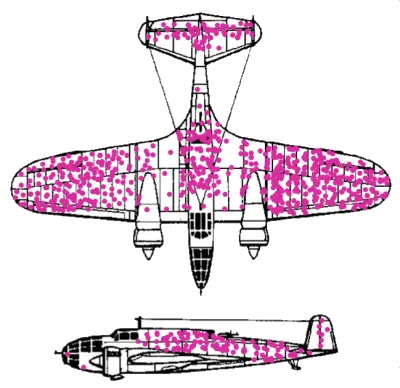
\includegraphics[width=0.5\linewidth]{img/bullet_holes_wwii}
	\caption{Bullet holes found in WWII allied bombers which returned after sorties}
	\label{fig:bulletholeswwii}
\end{figure}

\subsubsection{Cause-and-Effect Diagram}
This tool has the form of a fishbone diagram and is used for the systematic identification of causes resulting in problems.

\subsection{Control Charts}
The basis for control charts is the idea that a process can run according to specifications or outside of them. These are upper and lower bound and are derived statistically. The process is then continuously monitored and plotted against these bounds.

\subsubsection{Construction of Control Charts}
Periodic sampling of fixed sample size $n$ from the current production of the machine. The new parts are then drawn in a scatter plot with a centreline $\mu_0$ and with upper and lower control limit for a given $\alpha$ which defines the \textbf{control area}. The mean values are then continuously plotted against the index of the current measurement in the scatter diagram. The problem is that the process standard deviation is unknown.

The distance between upper control limit (UCL) and lower control limit (LCL) is three times the standard deviation.
\begin{align*}
	\text{LCL} &= \mu_0 - z_q \frac{\sigma}{\sqrt{n}}\\
	\text{UCL} &= \mu_0 + z_q \frac{\sigma}{\sqrt{n}}
\end{align*}

\begin{figure}[H]
	\centering
	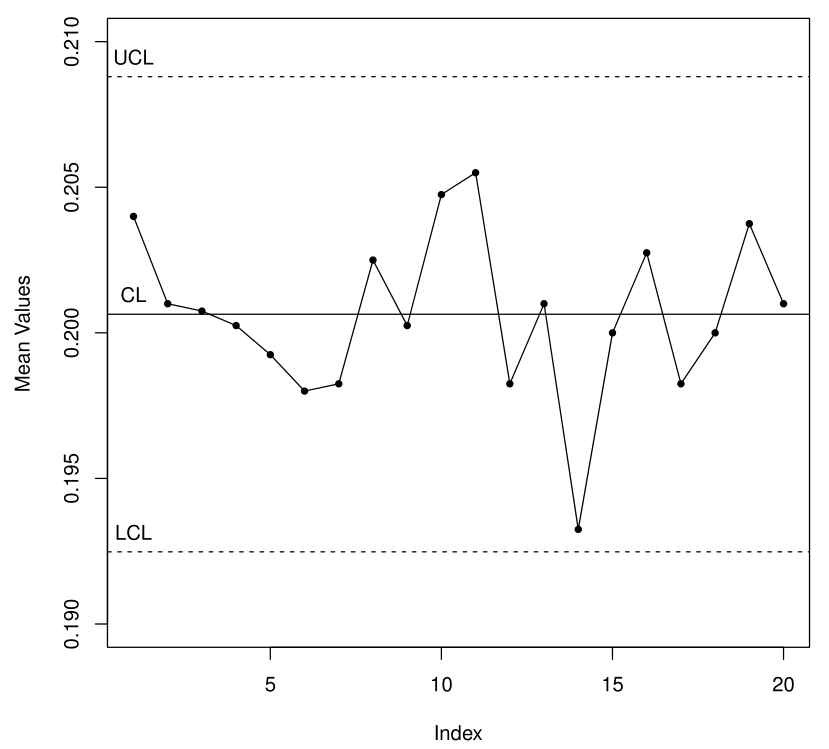
\includegraphics[width=0.5\linewidth]{img/control_chart}
	\caption{Sample control chart with UCL and LCL indicated}
	\label{fig:controlchart}
\end{figure}

\subsubsection{Shewhart Control Charts}
The problem with constructing the control chart is that mean and standard deviation of a process are generally unknown. Shewhart solves this by first monitoring the variation and then the mean of a process. Sample the process periodically under the assumption that the process is normally distributed.
\begin{enumerate}
	\item Calculate the mean of each sample
	\begin{equation*}
		\samplemean{x}_i = \frac{1}{n}\sum_{j=1}^{n}x_{ij}
	\end{equation*}
	\item Calculate standard deviation of the samples
	\begin{equation*}
		s_i = \sqrt{\frac{1}{n-1} \sum_{j=1}^{n}(x_{ij}-\samplemean{x}_i)^2}
	\end{equation*}
	\item Calculate the range R for each sample
	\begin{equation*}
		R_i = \max(x_{ij}) - \min(x_{ij}) \qquad j\in1..n
	\end{equation*}
\end{enumerate}

\paragraph{Construction of an $R$ chart} Take the data from the trial run with $k$ samples of sample size $n$ from the process under supervision. The centreline (CL) of the process is denoted by $\samplemean{R}$ and calculated as follows
\begin{equation*}
	\samplemean{R} = \frac{1}{k}\sum_{i=1}^{k}R_i
\end{equation*}
The standard deviation of the statistic $\samplemean{R}$ is denoted $\sigma_R$. The control limits of the $R$ chart can then be calculated
\begin{align}
	\text{LCL} &= D_3\samplemean{R}\\
	\text{UCL} &= D_4\samplemean{R}\\
\end{align}
The constants $D_3$ and $D_4$ are dependent on the sample size $n$ and must be looked up in a specific table.

After the centreline and the control limits are determined the ranges $R_i$ are sequentially entered against the index $i$ in a scatter plot. In addition, lines for the control limits UCL and LCL are drawn into the same graph. If a sample is outside the control area, the sample is omitted and the limits recalculated.

\paragraph{Construction of an $\samplemean{x}$ chart} The control limits of an $\samplemean{x}$ chart are based on the three sigma limits of the empirical distribution of the statistic $\samplemean{x}$.

The control limits are then
\begin{align}
	\text{LCL} &= \mu - 3 \frac{\sigma}{\sqrt{n}}\\
	\text{UCL} &= \mu + 3 \frac{\sigma}{\sqrt{n}}
\end{align}
The assumption is that the $R$ chart is under statistical control and the real value of $\sigma$ can thus be approximated by
\begin{equation*}
	\hat{\sigma} = \frac{\samplemean{R}}{d_2}
\end{equation*}
as it is a reliable estimate for the process deviation. The constant $d_2$ is again dependent on the sample size $n$ and can be found in the table.

Any samples excluded for the construction of the $R$ chart, should also be disregarded for the construction of the $\samplemean{x}$ chart. This results in a data set of $k^\star$ valid samples and a corrected estimate for $\mu$
\begin{equation*}
	\samplemean{\samplemean{x}} = \frac{1}{k^\star}\sum_{i=1}^{k^\star}\samplemean{x}_i
\end{equation*}
and the corrected control limits
\begin{align*}
	\text{LCL} &= \samplemean{\samplemean{x}} - 3 \frac{\samplemean{R}}{d_2}\frac{1}{\sqrt{n}} \approx \samplemean{\samplemean{x}} - A_2\samplemean{R} \\
	\text{UCL} &= \samplemean{\samplemean{x}} + 3 \frac{\samplemean{R}}{d_2}\frac{1}{\sqrt{n}} \approx \samplemean{\samplemean{x}} + A_2\samplemean{R}
\end{align*}

\paragraph{Construction of $\samplemean{x}$ and $s$} As there are different ways to measure the variation of a process, a number of different control charts may be employed. One combination that is often used is the $\samplemean{x}$ and $s$ charts. The construction of these two is similar to $\samplemean{x}$ based on $R$, again, the variation is brought under control and then the process standard deviation is estimated using the $\samplemean{x}$ chart.

The centreline of the $s$ chart is denoted $\samplemean{s}$ and is calculated from the standard deviations $s_i$ of the $k$ samples as follows
\begin{equation*}
	\samplemean{s} = \frac{1}{k}\sum_{i=1}^{k} s_i
\end{equation*}
The control limits are then
\begin{align*}
	\text{LCL} &= B_3\samplemean{s}\\
	\text{UCL} &= B_4\samplemean{s}\\
\end{align*}
After the centre line and control limits are determined, the sample standard deviation and lines are plotted in a scatter diagram. Any observation falling outside the control area are omitted and the ranges recalculated.

\paragraph{Construction of $\samplemean{x}$ based on $s$} Using an $s$ chart that is \textbf{under control} the process standard deviation can be estimated by
\begin{equation*}
	\hat{\sigma} = \frac{\samplemean{s}}{c_4}
\end{equation*}
As before, Any samples that were excluded for construction of the $s$ chart should also be disregarded for the construction of the $\samplemean{x}$ chart.

The mean values of the resulting $k^\star$ samples give an estimation of $\mu$
\begin{equation*}
	\samplemean{\samplemean{x}} = \frac{1}{k^\star}\sum_{i=1}^{k^\star}\samplemean{x}_i
\end{equation*}
The control limits are then
\begin{align*}
	\text{LCL} &= \samplemean{\samplemean{x}} - 3 \frac{\samplemean{s}}{c_4}\frac{1}{\sqrt{n}} \approx \samplemean{\samplemean{x}} - A_3\samplemean{s}\\
	\text{UCL} &= \samplemean{\samplemean{x}} + 3 \frac{\samplemean{s}}{c_4}\frac{1}{\sqrt{n}} \approx \samplemean{\samplemean{x}} + A_3\samplemean{s}
\end{align*}

\subsubsection{Individuals Control Charts}
Often its not practical to pick several production pieces for a sample data set, for example if a process is very slow (for example Falcon Heavy Boosters) or if the difference of a repeated measurement cannot be attributed to the process variation, but to the measuring methods. In such situations, it is reasonable to construct a control chart for individual measurements.

The problem that arises is that the variability of the process cannot be estimated from a single measurement. The solution is to use a moving range
\begin{equation*}
	MR_i = \abs{x_{i+1} + x_i}\quad \forall i\in1..n-1
\end{equation*}
The process standard deviation can be estimated from the arithmetic mean of the moving ranges
\begin{equation*}
	\samplemean{MR} = \frac{1}{n-1}\sum_{i=1}^{n-1}MR_i
\end{equation*}
\begin{equation*}
	\hat{\sigma} = \frac{\samplemean{MR}}{d_2}
\end{equation*}
With $d_2$ dependent on the sample size $n$, which would be two in this case as two neighbouring samples were used to calculate the moving range.
The centreline $samplemean{x}$ is the arithmetic mean of the measured values
\begin{equation*}
	\samplemean{x} = \frac{1}{n}\sum_{i=1}^{n}x_i
\end{equation*}
And the control limits
\begin{align*}
	\text{LCL} &= \samplemean{x} - 3\frac{\samplemean{MR}}{d_2}\\
	\text{UCL} &= \samplemean{x} + 3\frac{\samplemean{MR}}{d_2}
\end{align*}

\subsubsection{$p$ Control Chart}
Often we are only interested if a product is usable or defective, which makes the proportion of defectives to tested a discrete random variable. Thus a control chart for attributes data, the $p$ chart, can be used. This chart is cheaper and easier to use, but needs a bigger sample size $n$ than the Shewhart charts.

\vspace{1em}
\noindent
An estimator of success probability is the relative frequency
\begin{equation*}
	\hat{p} = \frac{D}{n}
\end{equation*}
And the variance then
\begin{equation*}
	\Var{\hat{p}} = \frac{p(1-p)}{n}
\end{equation*}
The centre line and the control limits are again determined from a \textbf{stable trial run} with $k^\star$ valid samples. In the event that all $n_i$ are equal
\begin{align*}
	\samplemean{p} &= \frac{1}{k^\star}\sum_{i=1}^{k^\star}p_i\\
	\text{LCL} &= \samplemean{p} - 3 \sqrt{\frac{\samplemean{p}(1-\samplemean{p})}{n}}\\
	\text{UCL} &= \samplemean{p} + 3 \sqrt{\frac{\samplemean{p}(1-\samplemean{p})}{n}}
\end{align*}
In the event that not all $n_i$ are equal
\begin{align*}
	\samplemean{p} &= \frac{d_1 + d_2 + \dots + d_{k^\star}}{n_1 + n_2 + \dots + n_{k^\star}}\\
	\text{LCL}_i &= \samplemean{p} - 3 \sqrt{\frac{\samplemean{p}(1-\samplemean{p})}{n}}\\
	\text{UCL}_i &= \samplemean{p} + 3 \sqrt{\frac{\samplemean{p}(1-\samplemean{p})}{n}}
\end{align*}
The control limits now depend on the index $i$. It might happen that for small sample sizes $n_i$ the control limits $\text{LCL}_i$ are negative, which obviously makes no sense in the context of a probability, in thus correct $\text{LCL}_i$ to $0$.

\subsection{Statistical Properties of Control Charts}
At any given time $t_i$ ($i\in\{1,\dots,k\}$) extract the last $n_i$ parts produced by the machine, calculate the relevant statistic (arithmetic mean for $\samplemean{x}$ chart, range for $R$ chart), and enter the value of the statistic against the index $i$ as a point. If the point is between the control limits the process is \textbf{under control}, otherwise its \textbf{out of control} and the production should be interrupted and the process checked.

\subsubsection{Western Electric Rules}
\begin{enumerate}
	\item Any single data point falls outside the limit defined by UCL and LCL (beyond the $3\sigma$-limit).
	\item Two out of three consecutive points fall beyond the limit defined by $\frac{2}{3}$ UCL and $\frac{2}{3}$ LCL on the same side of the centreline (beyond the $2\sigma$-limit).
	\item  Four out of five consecutive points fall beyond the limit defined by $\frac{1}{3}$ UCL and $\frac{1}{3}$ LCL on the same side of the centreline (beyond the $1\sigma$-limit).
	\item Nine consecutive points fall on the same side of the centreline (a so called \textbf{run}).
\end{enumerate}

\begin{figure}[htb]
	\begin{subfigure}{0.45\linewidth}
		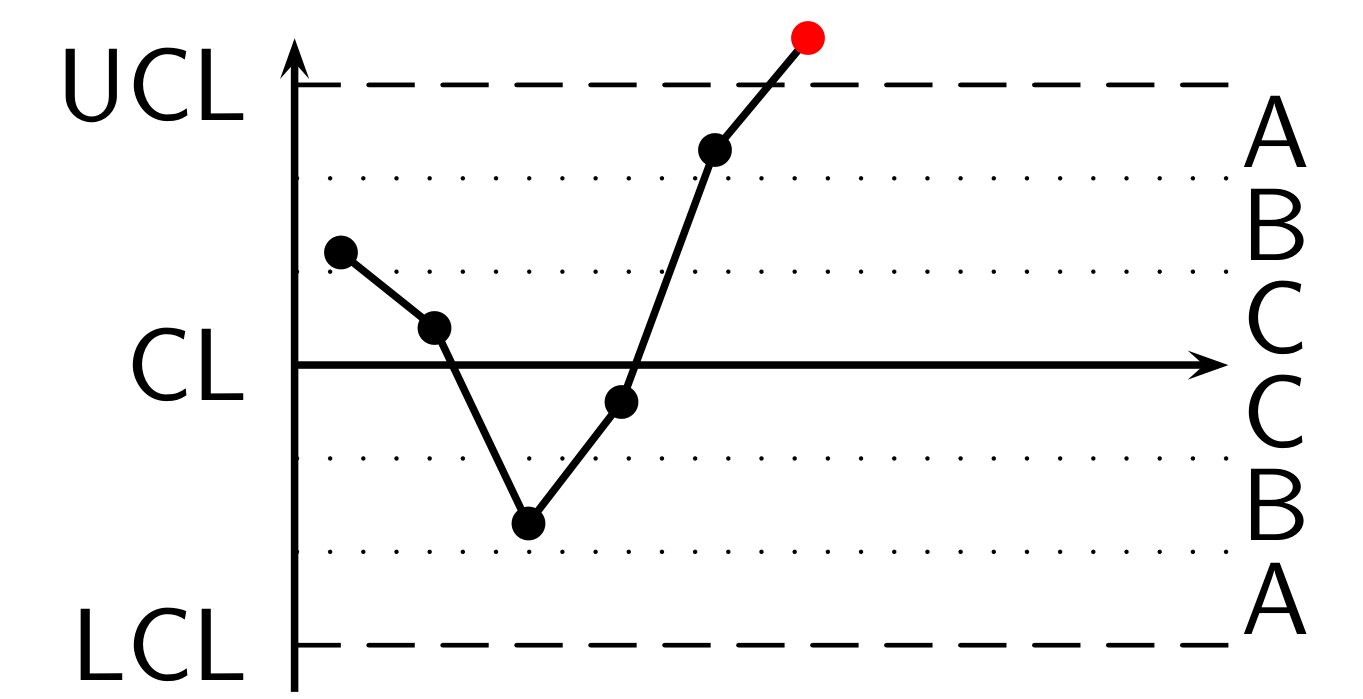
\includegraphics[width=\linewidth]{img/western_electric_rule1.png}
		\caption{Rule 1: Any point beyond zone A}
	\end{subfigure}
	\hfill
	\begin{subfigure}{0.45\linewidth}
		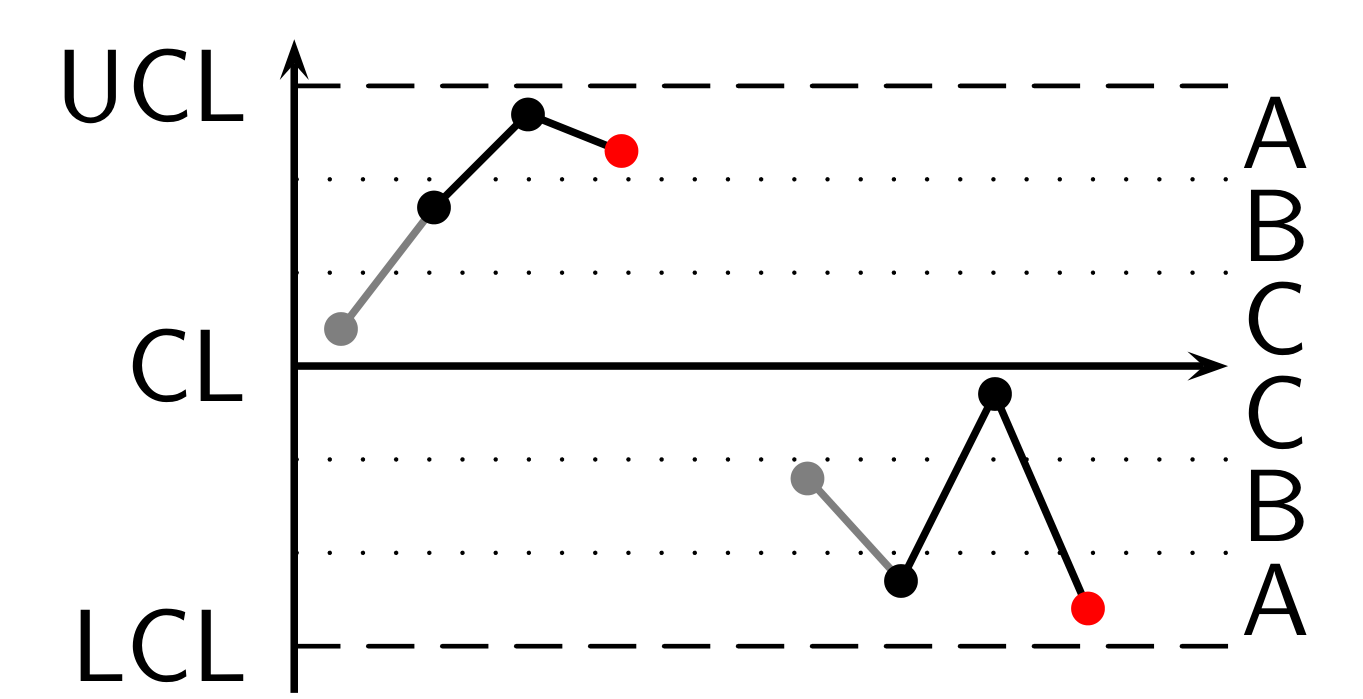
\includegraphics[width=\linewidth]{img/western_electric_rule2.png}
		\caption{Rule 2: Two out of three fall into zone A or beyond}
	\end{subfigure}
	\begin{subfigure}{0.45\linewidth}
		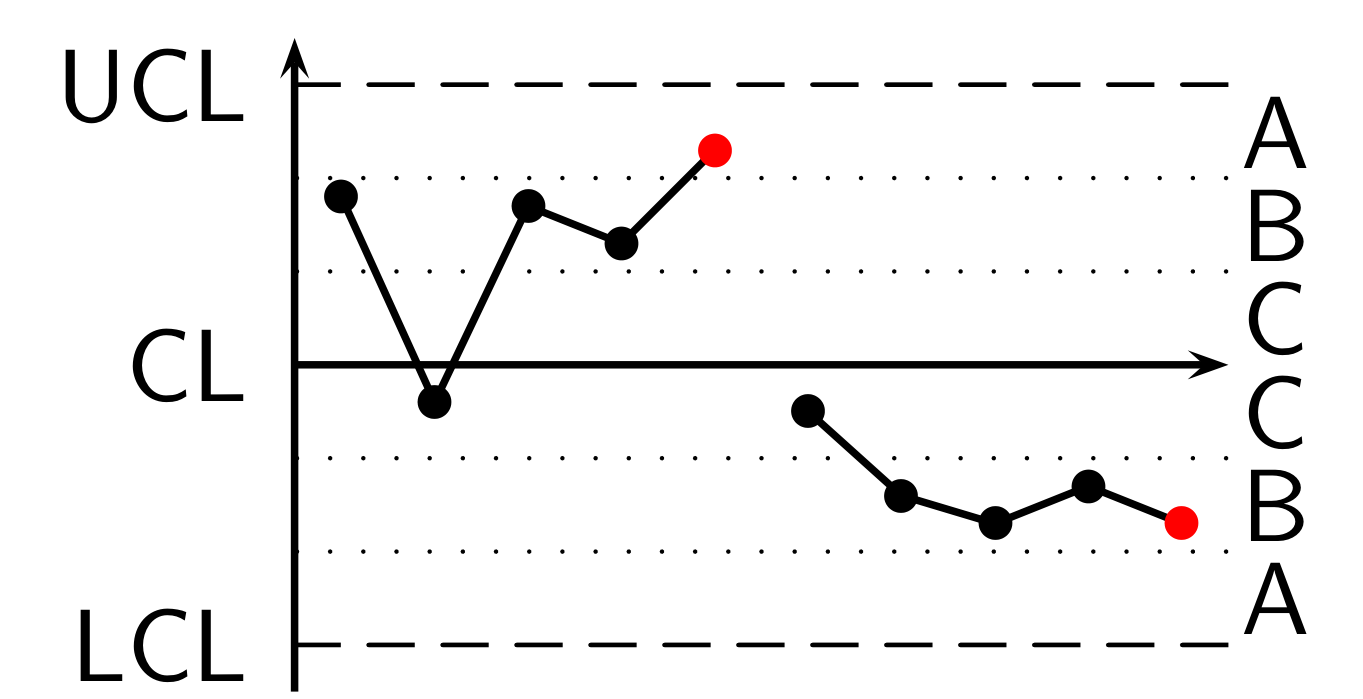
\includegraphics[width=\linewidth]{img/western_electric_rule3.png}
		\caption{Rule 3: 4 out of 5 consecutive points fall zone B or beyond}
	\end{subfigure}
	\hfill
	\begin{subfigure}{0.45\linewidth}
		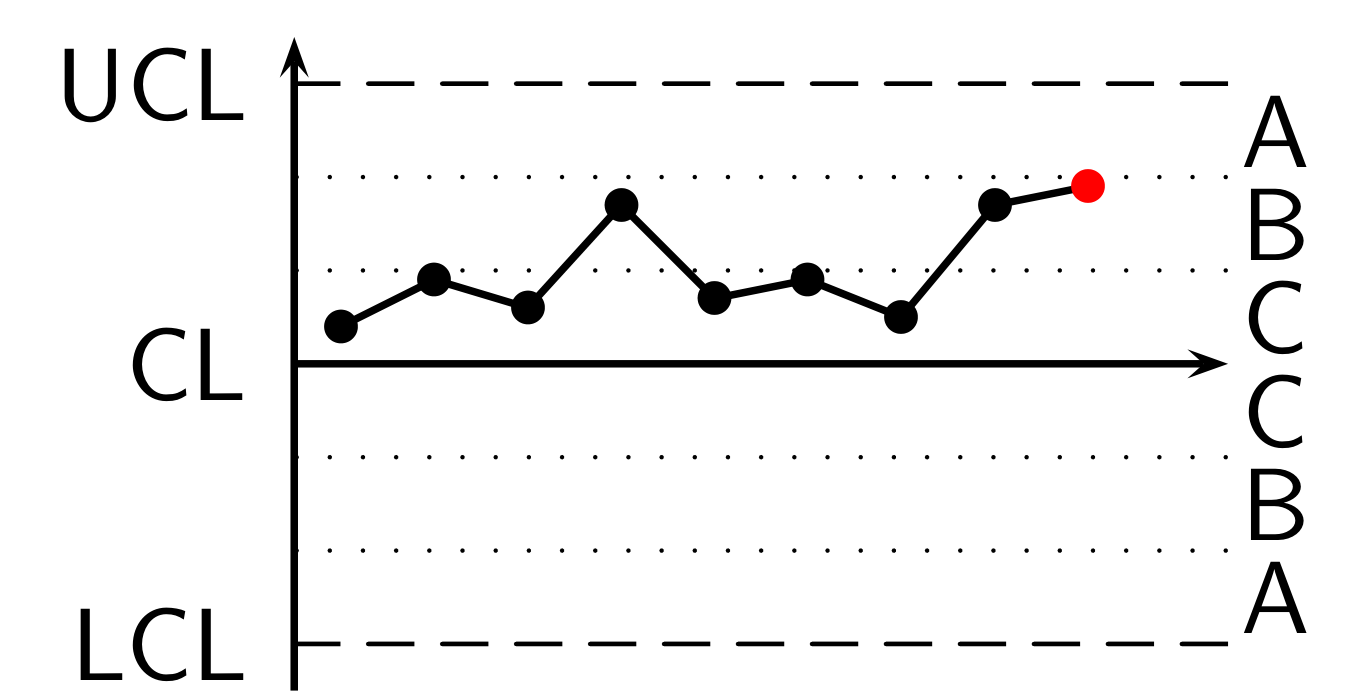
\includegraphics[width=\linewidth]{img/western_electric_rule4.png}
		\caption{Rule 4: 9 consecutive points fall on the same side of the centreline}
	\end{subfigure}
\end{figure}

\subsubsection{Type I and Type II Errors}
When monitoring a process with control charts there are two erroneous decisions one can make. If $\mu_0$ is the target value of a process, there are two hypotheses
\begin{itemize}
	\item[$H_0$:] $\mu_0 = \mu$, that is the process is not disturbed
	\item[$H_1$:] $\mu_0 \neq \mu$, that is the process is disturbed, $\mu_1$ is true
\end{itemize}
There are two errors one can make
\begin{enumerate}
	\item Type I: $H_0$ true, but is rejected (\textbf{false alarm})
	\item Type II: $H_0$ false, but is accepted (\textbf{omitted alarm})
\end{enumerate}

\begin{equation*}
	P(\text{Type I}) = \alpha
\end{equation*}

\begin{equation*}
	P(\text{Type II}) = \beta
\end{equation*}
$\beta$ depends on the true value of $\mu_1$ (which is unknown) and $n$.

\begin{figure}[H]
	\begin{subfigure}{0.48\linewidth}
		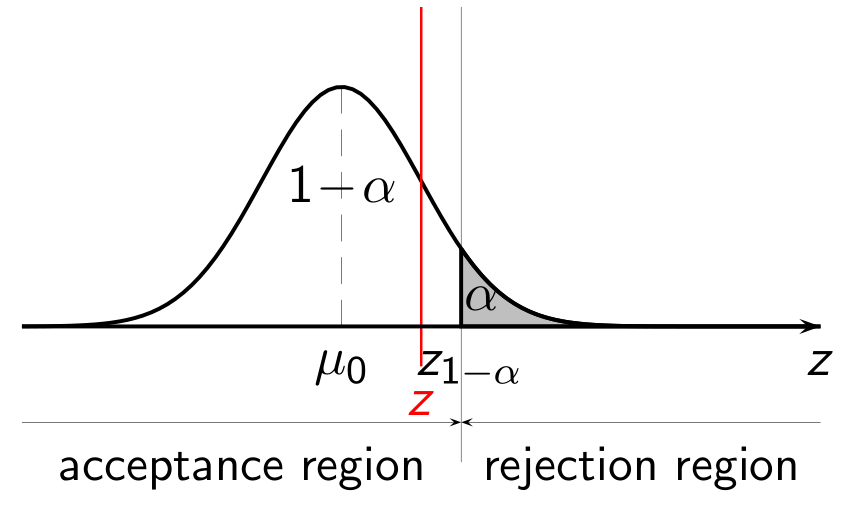
\includegraphics[width=\linewidth]{img/type_I_correct.png}
		\caption{Since $z < z_{1-\alpha}$ the null hypothesis is accepted. This is the right decision, which is made with probability $1 - \alpha$.}
	\end{subfigure}
	\hfill
	\begin{subfigure}{0.48\linewidth}
		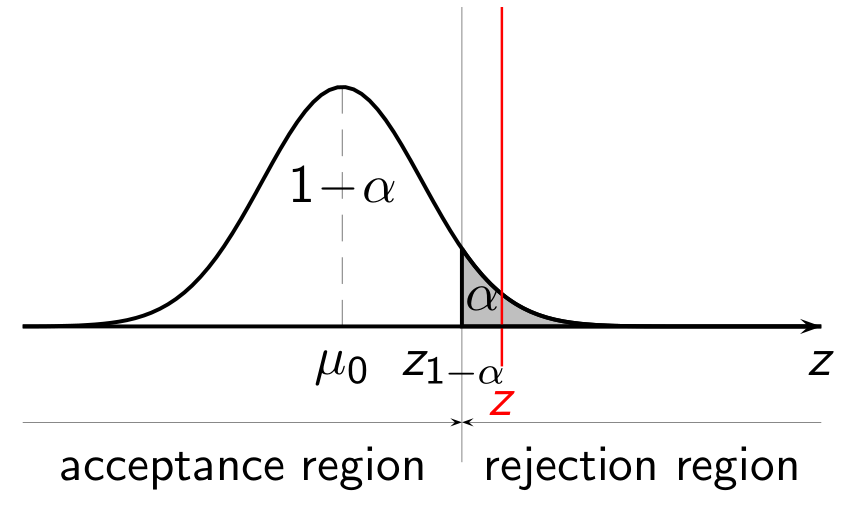
\includegraphics[width=\linewidth]{img/type_I_false.png}
		\caption{Since $z \geq z_{1-\alpha}$ the null hypothesis is rejected. This is the wrong decision (\textbf{type I error}), which is made with probability $\alpha$.}
	\end{subfigure}
	\caption{Outcomes when $H_0$ is true}
\end{figure}

\begin{figure}[H]
	\begin{subfigure}{0.48\linewidth}
		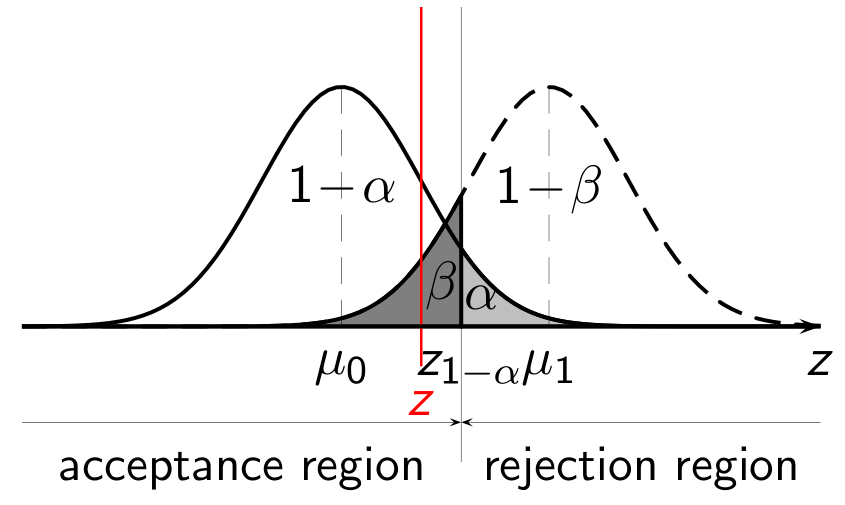
\includegraphics[width=\linewidth]{img/type_II_false.png}
		\caption{Since $z < z_{1-\alpha}$ the null hypothesis is accepted. This is the wrong decision (\textbf{type II error}), which is made with probability $\beta$.}
	\end{subfigure}
	\hfill
	\begin{subfigure}{0.48\linewidth}
		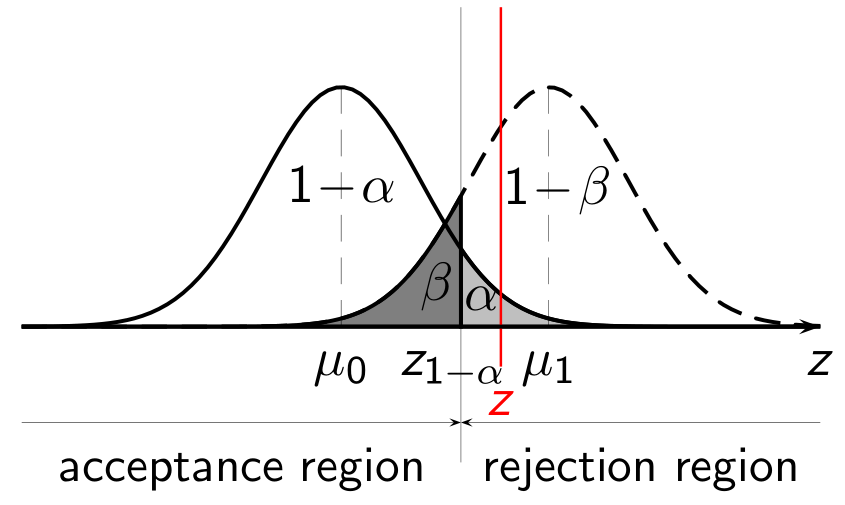
\includegraphics[width=\linewidth]{img/type_II_correct.png}
		\caption{Since $z \geq z_{1-\alpha}$ the null hypothesis is rejected. This is the correct decision, which is made with probability $1 - \beta$ (\textbf{power} of the test).}
	\end{subfigure}
	\caption{Outcomes when $H_0$ is false and alternative hypothesis $H_1$ (dashed density) is true}
\end{figure}

The power of a hypothesis test is the probability $1-\beta$ that the test correctly rejects the null hypothesis when the alternative hypothesis is true
\begin{equation*}
	\text{\textbf{power}} = P(\text{reject $H_0$}|\text{$H_1$ is true}) = 1 - \beta
\end{equation*}
The goal is to keep type I and type II errors small simultaneously, with the complicating factor that a reduction of $\alpha$ increases $\beta$ and vice versa.

\subsection{Power Function}
The power function is the probability of rejecting the null hypothesis $H_0$ if $H_1$ is true, that is the true distribution centres around $\mu_1$. This probability is clearly dependent on the location of $\mu_1$, but we are not interested in $\mu_1$ alone but in the the relation of $\mu_1$ to the target value $\mu_0$ and the process standard deviation $\sigma$. This gives a new normalised variable
\begin{equation*}
	\delta = \frac{\mu_1 - \mu_0}{\sigma}
\end{equation*}
This variable is a measure for the deviation of the observed, disturbed process from the undisturbed process in units of $\sigma$. In statistical process control the \textbf{power function} is denoted by
\begin{equation*}
	g(\mu_1) = g(\delta\sigma + \mu_0) = \tilde{g}(\delta)
\end{equation*}
and is a measure for the probability of intervening in a process.

\subsubsection{Ideal Power Function}
For an undisturbed process where $\mu = \mu_0$ it follows that
\begin{equation*}
	g(\mu_0) = \tilde{g}(0) = \alpha
\end{equation*}
where $\alpha$ is the error probability. In statistical process control $\alpha$ is $0.0027$. For a disturbed process $g(\mu_1)$ should be as large as possible and thus the probability for an omitted alarm $1-g(\mu_1)$ as small as possible. 

\subsubsection{Operating Characteristic}
The operating characteristic curve is the functional relation between the type II error and the position of $\mu_1$ or $\eta = \frac{\mu_1 - \mu_0}{\sigma}$ respectively
\begin{equation*}
	\text{OC}(\mu_1) = 1 - g(\mu_1)
\end{equation*}

\begin{figure}[H]
	\centering
	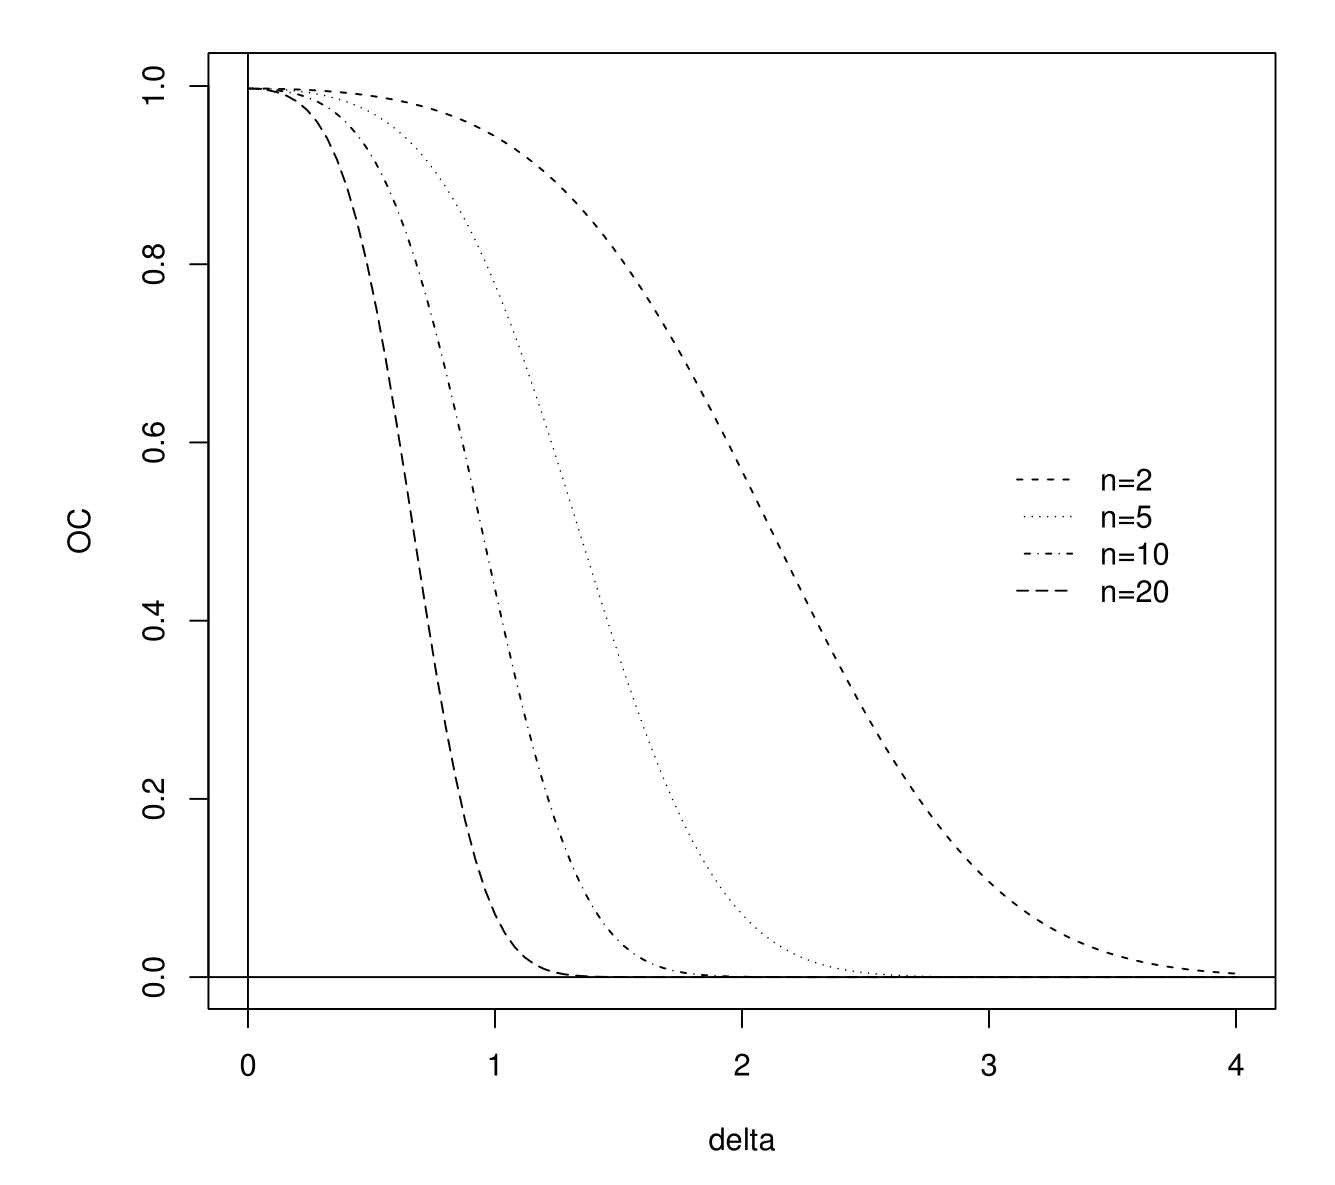
\includegraphics[width=0.4\linewidth]{img/OC_curve}
	\caption{An operating characeristic curve for different sample sizes $n$}
	\label{fig:occurve}
\end{figure}

\subsubsection{Average Run Length}
At every time $t_i$ with $i\in\{1,2,\dots,k\}$ a statistical test based on a random sample is made for the control chart. The assumption is to take $n$ random samples at fixed intervals and independent from the production process. The run length $I_{\text{RL}}$ is the time until an intervention in the production process is signalled. The run length is a discrete random variable, which takes values $k\in\{1,2,3,\dots\}$ with the probability
\begin{equation*}
	p_k = P(I_{\text{RL}} = k)
\end{equation*}
The expected value is called \textbf{average run length} (ARL)
\begin{equation*}
	\text{ARL} = \ev{I_{\text{RL}}} = \sum_{k=1}^{\infty} k\cdot p_k
\end{equation*}
The average run length is the mean time until the first intervention in the current process. It depends on the actual mean $\mu_1$ of the process and the control limits.

This chart would be ideal for an undisturbed process, that is $\mu = \mu_0$, thus no intervention or false alarm occurs
\begin{equation*}
	\text{ARL} = \ev{I_{\text{RL}}} = \infty
\end{equation*}
On the other hand, an immediate indication would be signalled with an ideal chart if the process is disturbed so far that an intervention is more economical than further production
\begin{equation*}
	\text{ARL} = \ev{I_{\text{RL}}} = 1
\end{equation*}

\paragraph{Calculation of the Average Run Length} The random variable $I_{\text{RL}}$ follows a geometric distribution with the probabilities
\begin{equation*}
	p_k = P(I_{\text{RL}} = k) = p\cdot(1-p)^{k-1}
\end{equation*}
where $p$ denotes the intervention probability and an expected value $\ev{I_{\text{RL}}} = \frac{1}{p}$.

The probability $p$ to intervene in the process depends on the actual process mean $\mu_1$ and on the control limits UCL and LCL.

\begin{equation*}
	p = p(\mu_1) = P(\mu\leq \text{LCL}) + P(\text{UCL} \leq \mu)
\end{equation*}

\begin{figure}[H]
	\centering
	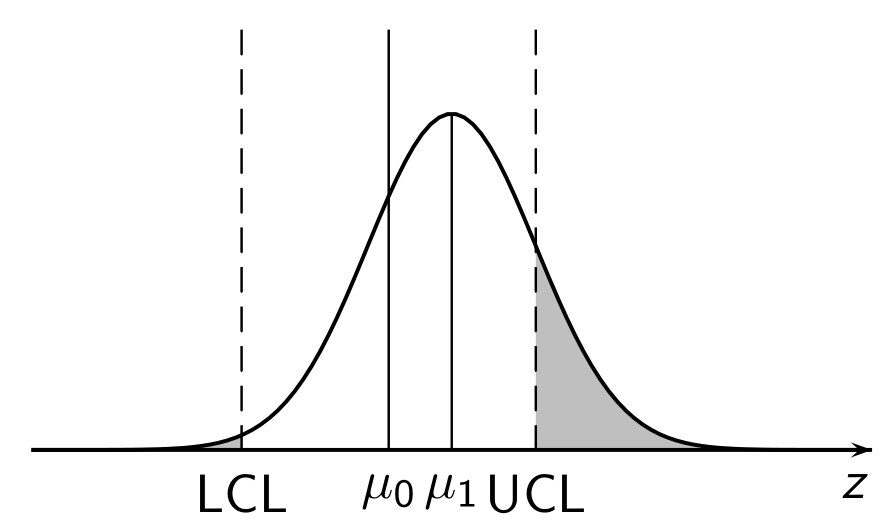
\includegraphics[width=0.6\linewidth]{img/average_run_length}
\end{figure}


\subsubsection{ARL versus Power Function}
The power function of the test is
\begin{equation*}
	p = p(\mu_1) = g(\mu_1) =\tilde{g}(\delta)\quad\text{with}\quad \delta=\frac{\mu_1-\mu_0}{\sigma}
\end{equation*}
Therefore the average run length is
\begin{equation*}
	\text{ARL}(\delta) = \frac{1}{g(\mu_1)} =\frac{1}{\tilde{g}(\delta)}
\end{equation*}
Instead of the power function, the average run length is also used to assess and compare different control charts.

\subsection{Process Capability}
The choice of the error probability $\alpha=0.0027$ implies that $99.73\%$ of all measured values, meaning almost all, lie within the three $\sigma$ range
\begin{equation*}
	[\mu_0 - 3\sigma, \mu_0 + 3\sigma]
\end{equation*}
However, the \textbf{control limits} $\text{LCL}=\mu_0 - 3\frac{\sigma}{\sqrt{n}}$ and $\text{UCL}=\mu_0 + 3\frac{\sigma}{\sqrt{n}}$ define a narrower zone.

\subsection{Tolerance Limits}
Technical tolerances for quality characteristics are defined in industry in the form of two tolerance limits
\begin{itemize}[nosep]
	\item \textbf{lower specification limit} (LSL), and
	\item \textbf{upper specification limit} (USL)
\end{itemize}
which have to be met in production.

If the measured value $x$ of the random variable $X$ is beyond the tolerance limits, then the part is rejected. And a control chart is only suitable for monitoring if the process produces as few rejects as possible.

The performance of a control chart is measured with so called \textbf{capability process ratios} (PCR). The simplest process capability index is
\begin{equation*}
	C_p = \frac{\text{USL} - \text{LSL}}{6\sigma}
\end{equation*}
The capability process ratio $C_p$ expresses the ratio of the width of the tolerance range to the width of the process range.

\vspace{1em}
\noindent
If the process is under control, that is $\mu_1 = \mu_0$ and $\text{SL} = \mu_0$, then $C_p = 1$ implies a reject rate of $\alpha\cdot100\% = 0.27\%$, $C_p < 1$ implies a reject rate greater than $\alpha\cdot100\% = 0.27\%$ and the process capability is \textbf{not} guaranteed, and $C_p > 1$ implies a reject rate less than $\alpha\cdot100\% = 0.27\%$ and the process capability \textbf{is} guaranteed.

In practice the target value $\mu_0$ and the process standard error $\sigma$ are unknown and estimated from a trial run. This results in an estimate for the process capability ratio, which is very sensitive if the process is not under control or the measured values are not normally distributed.

\subsection{Control Charts with Memory}
The decision to interfere with the manufacturing process with classical Shewhart control charts is based on the result of the current sample, and no consideration of the development of the manufacturing process in the past is made (except with the \textit{Western Electric rules}). The solutions is \textbf{modern control charts} with memory.

Given a data set with mean and standard deviation
\begin{tabularx}{\linewidth}{c | c c c c c c | c | c}
	sample & \multicolumn{6}{c |}{measured values} & mean & standard deviation\\
	\hline
	$1$ & $x_{11}$ & $x_{12}$ & $\dots$ & $x_{1j}$ & $\dots$ & $x_{1{\color{red}n_1}}$ & $\samplemean{x}_1$ & $s_1$ \\
	$2$ & $x_{21}$ & $x_{22}$ & $\dots$ & $x_{2j}$ & $\dots$ & $x_{2{\color{red}n_2}}$ & $\samplemean{x}_2$ & $s_2$ \\
	$\vdots$ & $\vdots$ & $\vdots$ &  & $\vdots$ & & $\vdots$ & $\vdots$ & $\vdots$ \\
	$i$ & $x_{i1}$ & $x_{i2}$ & $\dots$ & $x_{ij}$ & $\dots$ & $x_{i{\color{red}n_i}}$ & $\samplemean{x}_i$ & $s_i$ \\
	$\vdots$ & $\vdots$ & $\vdots$ &  & $\vdots$ & & $\vdots$ & $\vdots$ & $\vdots$ \\
	$k$ & $x_{k1}$ & $x_{k2}$ & $\dots$ & $x_{kj}$ & $\dots$ & $x_{k{\color{red}n_k}}$ & $\samplemean{x}_k$ & $s_k$ \\
\end{tabularx}
\begin{itemize}[nosep]
	\item Sample sizes $\color{red}n_i$ may be different
	\item Data comes from a normal distribution
\end{itemize}

\subsubsection{Memory}
The idea is to introduce a linear combination of the mean values $\samplemean{x}_j$ of samples from the past
\begin{equation*}
	y_i = \alpha_i + \sum_{j=1}^{i}\beta_j\samplemean{x}_j
\end{equation*}
where $\alpha_i$ and the weights $\beta_1,\dots,\beta_i$ can be arbitrary real numbers with the sum $\sum_{j=1}^{i}\beta_j = 1$.

\subsubsection{Cumulative Sum Control Chart (CUSUM)}
The idea being that the CUSUM chart plots the cumulative sums of deviations of measurement values from the target value. Given is the mean $\samplemean{x}_i$ of the $i$-th sample of a process, target value $\mu_0$ and the process standard deviation $\sigma$, which is known or estimated from the data.

The goal is to have a control chart that quickly detects a drift from the target value.

\paragraph{Construction of the Cumulative Sum Control Chart} The construction is a recursive procedure using two statistics $C^+$ and $C-$, which sum up the deviations above and below target value respectively
\begin{align*}
	C_i^+ &= \max\left\{0, C_{i-1}^+ + \samplemean{x}_i - (\mu_0 + K)\right\}\\
	C_i^- &= \max\left\{0, C_{i-1}^- - \samplemean{x}_i + (\mu_0 - K)\right\}
\end{align*}
with the starting values $C_0^+ = C_0^- = 0$. If a shift of $\Delta$ is to be detected, set $K=\frac{\Delta}{2}$. This constant $K$ is called \textbf{reference value}.

$C^+$ and $C^-$ only sum up deviations from the target value, which are greater than the reference value $K$. If the process is under control, that is for all $i$
\begin{equation*}
	\mu_0 - K \leq \ev{\samplemean{x}_i}\leq\mu_0+K,
\end{equation*}
then the expected values of the statistics are both zero.
\begin{equation*}
	\ev{C_i^+} = \ev{C_i^-} = 0
\end{equation*}
In this case the two random variables $C_i^+$ and $C_i^-$ fluctuate around the line at zero.

If the process is out of control beyond a certain index $i_0$
\begin{equation*}
	\ev{\samplemean{x}_i} = \mu \geq \mu_0 + K \forall i\geq i_0
\end{equation*}
then the statistic $C^+$ sums up the deviation from $\mu_0 + K$, that is 
\begin{align*}
	\ev{C_i^+} &\geq \left(\mu - (\mu_0 + k)\right)\cdot (i - i_0)\\
	\ev{C_i^-} &= 0
\end{align*}
From the moment $i_0$ where the disturbance occurs, the points $(i,C_i^+)$ lie on average above a straight line with slope $\mu - (\mu_0 + K)$. The same happens for $C^-$ if the process is not under control in the other direction.

The process is \textbf{out of control} if either $C^+$ or $C^-$ exceed a constant $H$, which is called the \textbf{decision interval}. If the process is out of control, it is stopped and the cause investigated. After the problem has been resolved, the CUSUM is restarted from zero.

\paragraph{Choice of $K$ and $H$} As the CUSUM should still have a good ARL, this choice is important. As a rule of thumb, with $\hat{\sigma}$ being an estimate of the process standard deviation
\begin{align*}
	K &= \frac{\hat{\sigma}}{2} \tag{reference value}\\
	H &= 5\hat{\sigma} \tag{decision interval}
\end{align*}

\subsubsection{Exponentially Weighted Moving Average (EWMA)}
The idea is to still monitor the means but have their weights $\beta_j$ decay exponentially. Given are the mean $\samplemean{x}_i$ of the $i$-th sample of a process, the target value $\mu_0$ and the process standard deviation $\sigma$, which is either known or estimated from the data. The goal is to have a control chart that quickly detects a drift from the target value.

\begin{align*}
	\lambda&: 0\leq\lambda\leq 1 \tag{smoothing paramater}\\
	y_i &= \alpha_i + \sum_{j=1}^{i}\beta_j\samplemean{x}_j\\
	\intertext{\textbf{Weights:}}
	\alpha_i &= (1 - \lambda)^i \cdot \mu_0\\
	\beta_j &= \lambda\cdot(1-\lambda)^{i-j}\quad\text{with}\quad j\in\{1,2,\dots,i\}
	\intertext{\textbf{Statistic:}}
	y_i &= (1-\lambda)^i \mu_0 + \lambda\sum_{j=1}^{i}(1-\lambda)^{i-j} \samplemean{x}_j
\end{align*}

\paragraph{Construction of an EWMA Chart} The EWMA chart is constructed in a recursive fashion.
\begin{align*}
	y_0 &= \mu_0 \tag{Initialisation}\\
	y_i &= (1-\lambda)y_{i-1} + \lambda\cdot\samplemean{x}_i \tag{Recursion}
\end{align*}

The \textbf{smoothing parameter} $\lambda$ determines the influence of the previous sample mean $\samplemean{x}_j$ on the statistic
\begin{equation*}
	y_i = (1-\lambda)^i\cdot\mu_0 + \lambda\cdot\sum_{j=1}^{i}(1-\lambda)^{i-j}\samplemean{x}_j
\end{equation*}
The smaller this smoothing parameter is the more previous sample means are used for the decision. The EMWA has thus a non-constant, unlimited memory. If the process is under control, then $\samplemean{x}_i$ comes from a normal distribution with the expected value $\mu_0$ and the standard deviation $\frac{\sigma}{\sqrt{n}}$, whereby the standard deviation is either known or estimated from data. The statistic $y_i$ is then also normally distributed with
\begin{align*}
	\ev{y_i} &= \mu_0
	\intertext{and}
	\Var{y_i} &= \frac{\lambda}{2-\lambda}\left(1 - (1-\lambda)^{2\cdot i}\right)\frac{\sigma^2}{n}
\end{align*}
This results in the $3\sigma$ control limits
\begin{align*}
	\text{LCL}_i = \mu_0 - 3\frac{\sigma}{\sqrt{n}}\sqrt{\frac{\lambda}{2-\lambda}\left(1 - (1-\lambda)^{2\cdot i}\right)}
	\intertext{and}
	\text{UCL}_i = \mu_0 + 3\frac{\sigma}{\sqrt{n}}\sqrt{\frac{\lambda}{2-\lambda}\left(1 - (1-\lambda)^{2\cdot i}\right)}
\end{align*}
A small $i$ results in \textbf{asymptotic control limits}
\begin{align*}
	\text{LCL}_i = \mu_0 - 3\frac{\sigma}{\sqrt{n}}\sqrt{\frac{\lambda}{2-\lambda}}
	\intertext{and}
	\text{UCL}_i = \mu_0 + 3\frac{\sigma}{\sqrt{n}}\sqrt{\frac{\lambda}{2-\lambda}}
\end{align*}
With the \textbf{estimate of the process standard error} $\hat{\sigma}=\frac{\samplemean{s}}{c_4}$ (the factor $c_4$ can be found in table \ref{tbl:FactorsControlCharts}).

\subsection{Acceptance Sampling}
This is a topic of statistical quality control. Certain products can't all be tested, as they get used up during testing (for example single use syringes or bullets). As a compromise draw random samples and make a decision on the quality of the population based on this information.
\begin{itemize}[leftmargin=*, labelindent=3cm, labelsep=0.5cm]
	\item[Lot:] Bulk of a product produced under \textbf{constant conditions}
	\item[Quality Control:] Accept or reject a lot
\end{itemize}
The tool to do this is an acceptance sampling plan. An important remark to make is, that with acceptance sampling one cannot directly intervene in the production process, but only decide whether to accept a delivery or production batch.
\begin{definition}
	An \textbf{acceptance sampling plan} is a set of instructions to decide on the acceptance or return of a lot.
\end{definition}
There are two kinds of acceptance sampling
\begin{itemize}
	\item sampling plans for attributes (counting)
	\item sampling plans for variables (measuring)
\end{itemize}

\subsubsection{Acceptance Sampling Plans for Attributes}
Given a lot with $N$ units called a population of which $m$ are defective parts with $0\leq m\leq N$. Then the percentage of defective parts is
\begin{equation*}
	p = \frac{m}{N}
\end{equation*}
In reality the number of defective parts $m$ and thus the percentage of defective parts $p$ are unknown. The goal is thus to estimate $p$ and to decide whether to accept or reject the lot with the help of a random sample of sample size $n\leq N$. Let $x$ be the number of defective units in the the sample with size $n$.
The acceptance sampling plan consists of the sample size $n$, the acceptance number $c$ and a rule
\begin{itemize}[nosep]
	\item $x\leq c$, then the lot is accepted
	\item $x>c$ the the lot is rejected
\end{itemize}
This procedure corresponds to a statistical hypothesis test (one sided)
\begin{itemize}
	\item $H_0: p=\frac{c}{n}$
	\item $H_1: p>\frac{c}{n}$
	\item Statistic: $X = \#\text{defective units in sample}\in\{0,\dots,n\}$
\end{itemize}
Reject $H_0$ if $\frac{x}{n}>\frac{c}{n}\Leftrightarrow x>c$. Of course errors can be made here too
\begin{itemize}
	\item Type I Error: $H_0$ is true but gets rejected with probability $\alpha = P(x>c)$ (producer's risk)
	\item Type II Error: $H_1$ is true but $H_0$ is accepted with probability $\alpha = P(x\leq c)$ (consumer's risk)
\end{itemize}

% TODO Write lecture slides in here

\subsubsection{Operating Characteristic}
The operating characteristic curve plots the probability of accepting a lot as a function of the percent defective $p$. $OC(p)$ is the probability of accepting a lot given that the true percent defective is $p$, called the acceptance probability with $P(X\leq c)$ for $p\in[0,1]$ (depends on $n$ and $c$).

\vspace{0.5em}
\noindent
\textbf{Properties}
\begin{itemize}
	\item Decreases with $p$
	\item $OC(0) = 1$ and $OC(1) = 0$
\end{itemize}
In the extreme case of total control and complete information $n=N$ one gets the ideal OC curve
\begin{figure}[H]
	\centering
	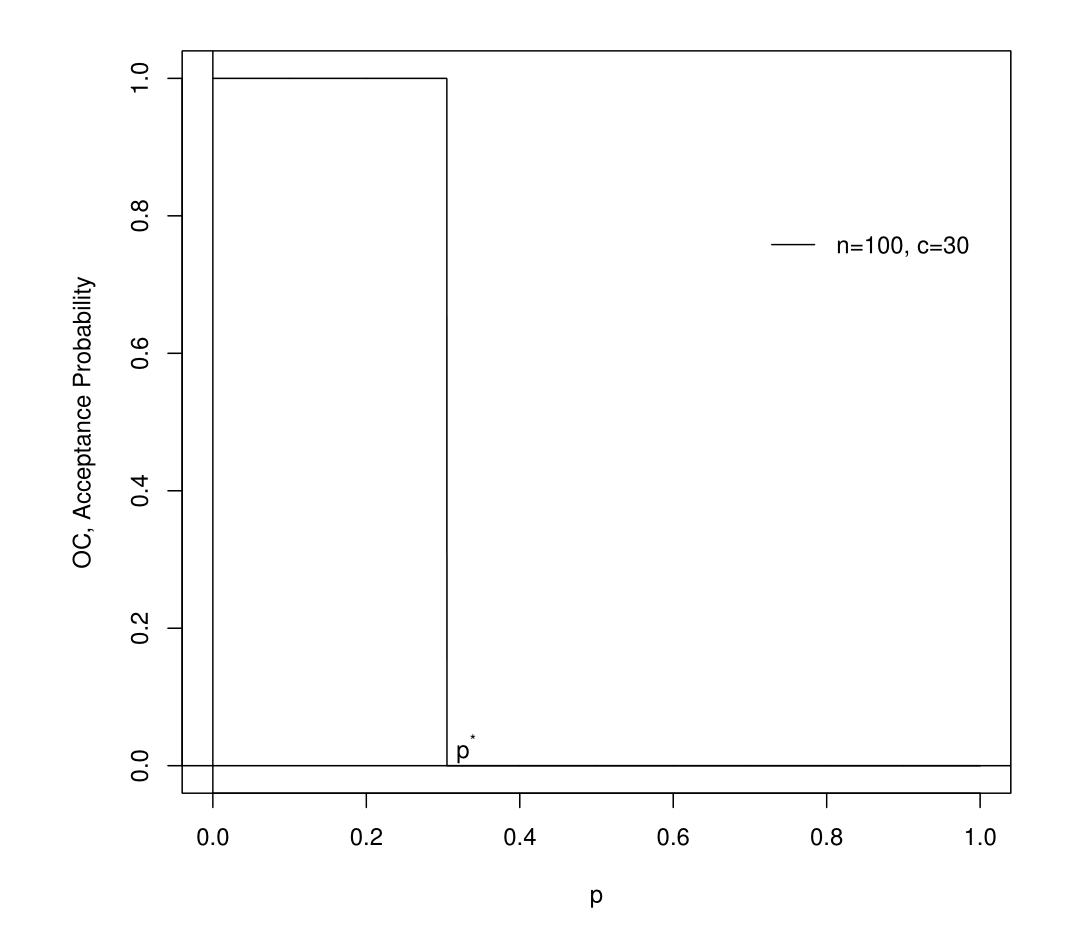
\includegraphics[width=0.5\linewidth]{img/ideal_OC_curve}
\end{figure}
But usually $n<N$ and the ideal OC curve is not achievable, but should be approached as closely as possible.
\begin{equation*}
	OC(p) = P(X\leq c) = \sum_{k=0}^c P(X=k) = \sum_{k=0}^c \frac{\binom{pN}{k}\cdot\binom{N-pN}{n - k}}{\binom{N}{n}}
\end{equation*}

\subsubsection{Find Parameters of Acceptance Sampling Plan}
The goal is to find the parameters $n$ and $c$ of the acceptance sampling plan, with the restriction that the sample size $n$ and the acceptance number $c$ have to be natural numbers with $0\leq c<n \leq N$. The OC curve depends on the parameters and increases with $c$ and decreases with $n$ given a constant $p$.

The requirements given by the opposing parties are
\begin{itemize}
	\item Producer: $OC(p_\alpha) \geq 1-\alpha$
	\item Consumer: $OC(p_\beta) \leq \beta$
\end{itemize}
This results in two points, the \textbf{producer's risk point} $(p_\alpha, 1-\alpha)$ and \textbf{consumer's risk point} $(p_\beta, \beta)$
\begin{figure}[H]
	\centering
	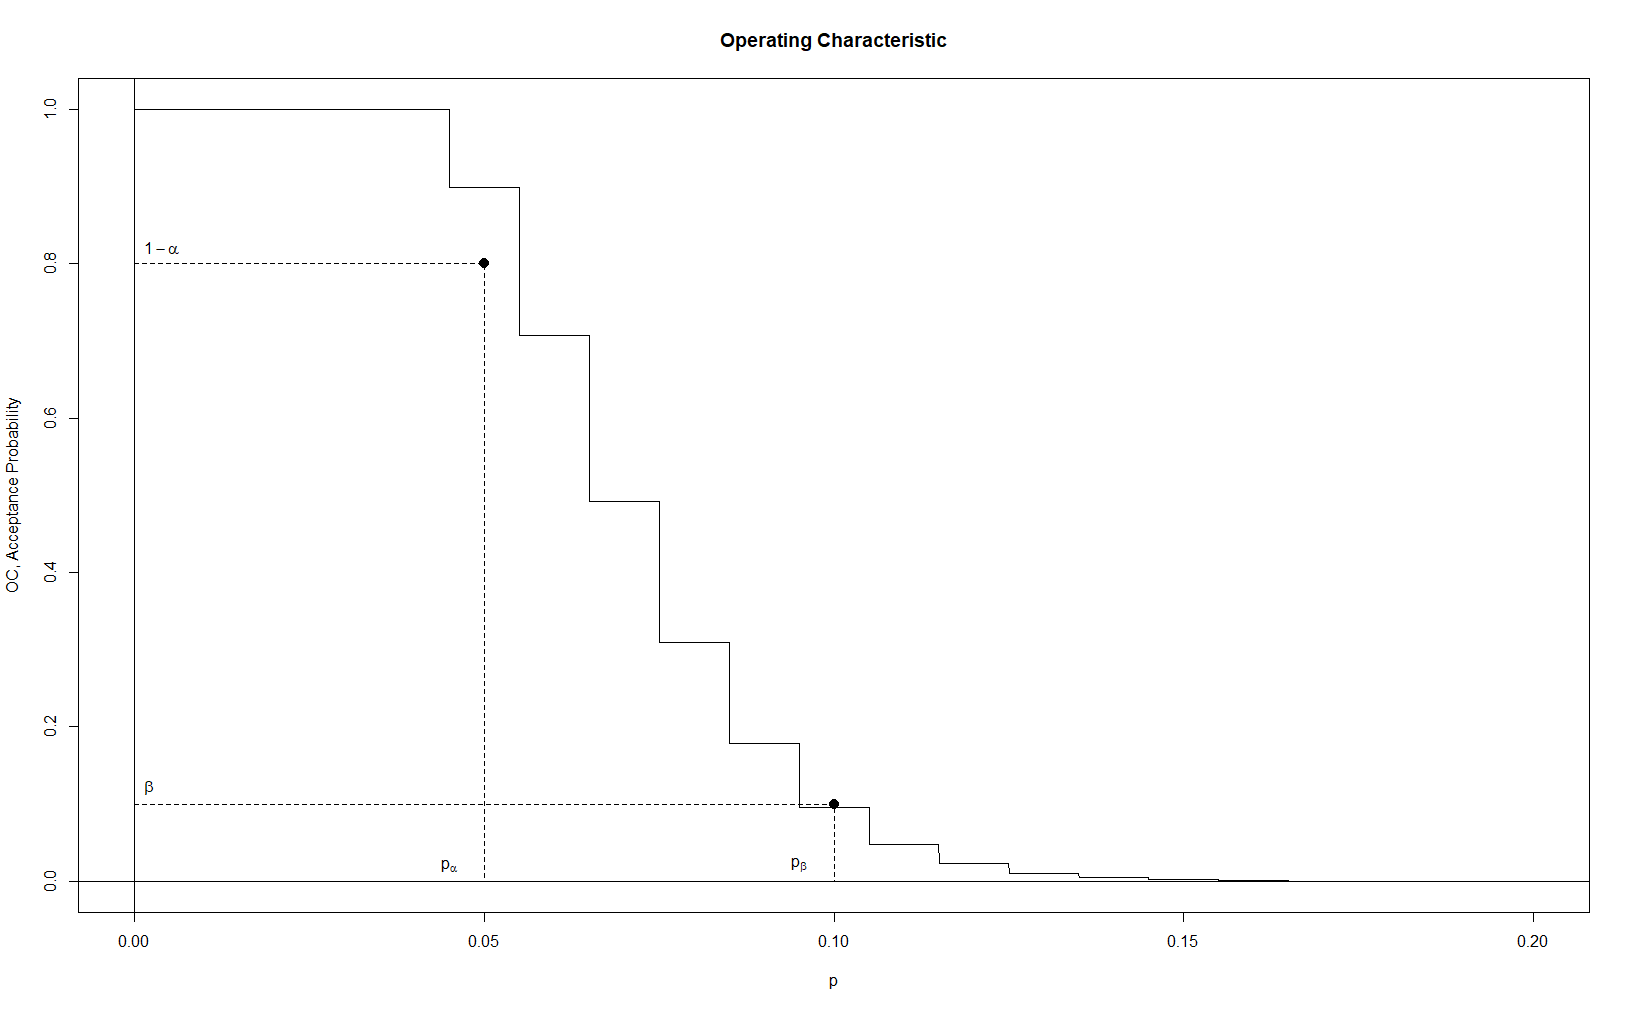
\includegraphics[width=0.8\linewidth]{img/OC_curve_points.png}
	\caption{Sample operating characteristics curve with risk points}
\end{figure}

\subsubsection{R}
For the operating characteristic the hypergeometric distribution is used as \textit{the hypergeometric distribution is used for sampling without replacement}. The density of this distribution with parameters $m, n$ and $k$ (named $Np$, $N-Np$, and $n$, respectively in the reference below, where $N := m+n$ is also used in other references) is given by 
\begin{equation*}
	p(x) = \frac{\binom{m}{x}\binom{n}{k-x}}{\binom{m+n}{k}}
\end{equation*}

In addition we use the function \mintinline{R}{phyper(q,m,n,k)} the following way
\begin{minted}{R}
func.OC <- function(p,N,n,c) { phyper(q=c, m=p*N, n=(1-p)*N, k=n) }
\end{minted}

\section{Multiple Regression}

\subsection{Simple Linear Regression Model}
This model has a single predictor variable which has an effect on the response that conforms to a straight line. It is the most important and widely used statistical technique and helps in the investigation and modelling of relationships between variables.

\subsubsection{Basic Model}
\begin{equation*}
	y = \beta_0 + \beta_1 x + \varepsilon
\end{equation*}
\begin{itemize}
	\item Predictor variable $x$
	\item Response variable $y$
	\item Random error term $\varepsilon$ with $\ev{\varepsilon} = 0$ and $\Var{\varepsilon} = \sigma^2$
\end{itemize}

% TODO Write down lecture slide note

\subsubsection{Remarks}
The regression equation is in real applications only an approximation to the true functional relationship between the variables of interest.
\begin{itemize}
	\item The regression equations summarise or describe the data set
	\item Predictions, forecasts, inter- or extrapolation are always done with a confidence interval
	\item Reduction of the complexity of a model by omitting unimportant variables
	\item Searching for optimal production conditions
\end{itemize}

\subsubsection{Data Set and Model}
Given a data set of $n$ points
\begin{equation*}
	(x_1,y_1), (x_2,y_2), \dots, (x_n,y_n)
\end{equation*}
and the model
\begin{equation*}
	y = \beta_0 + \beta_1 x + \varepsilon
\end{equation*}
find the parameters $\beta_0$, $\beta_1$ and $\sigma^2$ such that the model fits the data as well as possible.

\vspace{1em}
\noindent
Minimise:
\begin{equation*}
	S(\beta_0, \beta_1) = \sum_{i=1}^{n} \left(y - (\beta_0 + \beta_1 x_i)\right)^2
\end{equation*}
With $\hat{\beta}_0$ and $\hat{\beta}_1$ being the least-squares estimators of $\beta_0$ and $\beta_1$ respectively, taking the partial derivatives and solving for $0$ results in intercept and slope
\begin{align*}
	\hat{\beta}_0 &= \frac{\frac{1}{n}\sum_{i=1}^{n} x_i^2 \sum_{i=1}^{n}y_i - \frac{1}{n}\sum_{i=1}^{n} x_i^2 \sum_{i=1}^{n}x_i y_i}{\sum_{i=1}^{n}x_i^2 - \frac{1}{n}\left(\sum_{i=1}^{n}\right)^2}\\
	\hat{\beta}_1 &= \frac{\sum_{i=1}^{n}x_i y_i - \frac{1}{n}\sum_{i=1}^{n}x_i\sum_{i=1}^{n}y_i}{\sum_{i=1}^{n}x_i^2 - \frac{1}{n}\left(\sum_{i=1}^{n}\right)^2}
\end{align*}
The residuals are the difference between the observed values and their fitted value
\begin{equation*}
	e_i = y_i - (\hat{\beta}_0 + \hat{\beta}_1 x_i)
\end{equation*}
The expected mean of $e$ is zero
\begin{equation*}
	\samplemean{e} = \frac{1}{n}\sum_{i=1}^{n}\left(y_i - (\hat{\beta}_0 + \hat{\beta}_1 x_i)\right) = 0
\end{equation*}
The error sum of squares is an unbiased estimator for the variance $\sigma^2$ if it is divided by $n-2 $ degrees of freedom
\begin{equation*}
	\sigma^2 = \frac{1}{n-2} \sum_{i=1}^{n} e_i^2
\end{equation*}
The implicit assumption is that all errors $\varepsilon_i$ are normally distributed with expected value $0$ and variance $\sigma^2$, and the estimators $\hat{\beta}_0$ and $\hat{\beta}_1$ are normally distributed with
\begin{align*}
	\hat{\beta}_0 &\sim \N{\beta_0, \sigma^2\left(\frac{1}{n}+\frac{\samplemean{x}^2}{S_{xx}}\right)}\\
	\hat{\beta}_1 &\sim \N{\beta_1, \frac{\sigma^2}{S_{xx}}}
\end{align*}
where $S_{xx} = \sum_{i=1}^{n}(x_i - \samplemean{x})^2$

\subsubsection{Statistical Test on the Slope}
Alternative hypotheses:
\begin{align*}
	H_0 &: \beta_1 = \beta_{1,0}\\
	H_1 &: \beta_1 \neq \beta_{1,0}
\end{align*}
Test statistic:
\begin{equation*}
	T = \frac{\hat{\beta}_1 - \beta_{1,0}}{\se{\hat{\beta}_1}}
\end{equation*}
with the standard error
\begin{equation*}
	\se{\hat{\beta}_1} = \sqrt{\frac{\hat{\sigma}=2}{S_{xx}}}\quad\text{with}\quad S_{xx} = \sum_{i=1}^{n}(x_i - \samplemean{x})^2
\end{equation*}

Under the null hypothesis the test statistic $T$ follows a Student's $t$-distribution with $n-2$ degrees of freedom. The $p$-value is the probability, that under the null hypothesis, obtaining a result equal to or more extreme than what was actually estimated. The $p$-value for the two-sided alternative is
\begin{equation*}
	p = P(\beta_1 \leq \abs{\hat{\beta}_1} | H_0\text{ is true}) + P(\abs{\hat{\beta}_1} \leq \beta_1 | H_0\text{ is true})
\end{equation*}
\begin{center}
	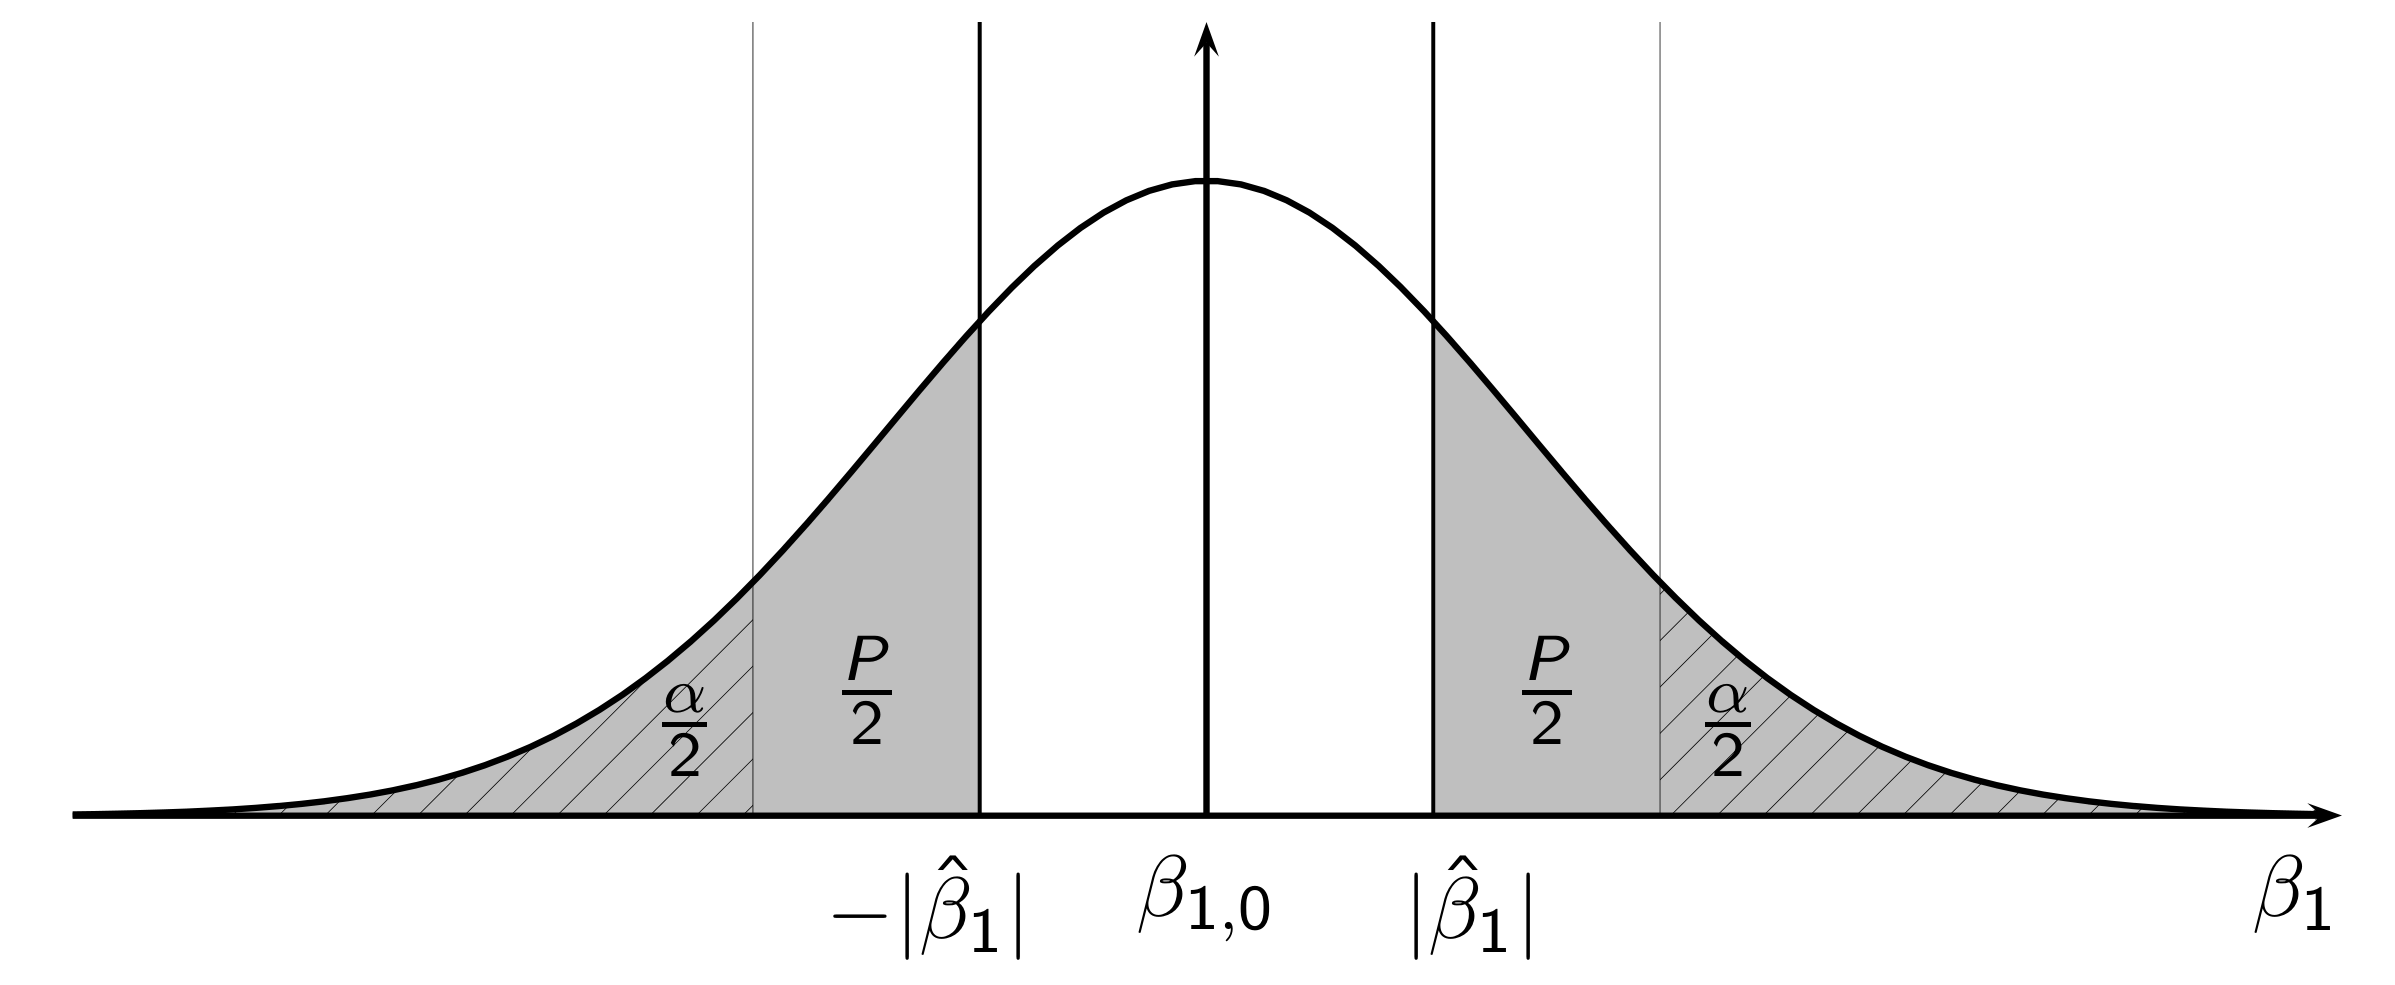
\includegraphics[width=0.8\linewidth]{img/p_value}
\end{center}

\paragraph{Remarks} The idea of a statistical test is to determine if a model can be true or not. The test is a rule that decides which scenario is more probable. The most plausible value for the parameters is the \textbf{least squares estimator}, and if a certain value is plausible is based on a statistical hypothesis test. However, a multitude of values are overall plausible, these form the \textbf{confidence interval}.

\subsubsection{Confidence Interval on the Slope}
The test statistic $ T = \frac{\hat{\beta}_1 - \beta_{1,0}}{\se{\hat{\beta}_1}}$ is accepted on the significance level $\alpha$ if
\begin{equation*}
	t_{\frac{\alpha}{2}, n-2} \leq T \leq t_{1 - \frac{\alpha}{2}, n-2}
\end{equation*}
This is called the \textbf{region of acceptance}. The \textbf{confidence interval on the slope} is
\begin{equation*}
	\hat{\beta}_1 - t_{\frac{\alpha}{2}, n-2}\cdot\se{\hat{\beta}_1} \leq \beta_1 \leq \hat{\beta}_1 + t_{1-\frac{\alpha}{2}, n-2}\cdot\se{\hat{\beta}_1}
\end{equation*}
The width of this confidence interval is a measure of the overall quality of the regression line.

\subsubsection{Confidence Interval on the Response}
The prediction interval will be wider than the confidence interval on the response as the variance of future observations has to be considered too. During the application of a regression model the response $y$ gets estimated for a particular value of the explanatory variable $x$. The \textbf{estimated response} is
\begin{equation*}
	\hat{y}_0 = \hat{\beta}_0 + \hat{\beta}_1 x_0
\end{equation*}
The confidence interval of the response is related to the null hypothesis $H_0: \hat{y}_0 =\mu_0$. The estimator $\hat{y}_0$ is normally distributed and unbiased with
\begin{equation*}
	\Var{\hat{y}_0} = \sigma^2\left(\frac{1}{n} + \frac{(x_0 - \samplemean{x})}{S_{xx}}\right)
\end{equation*}
Giving the test statistic of the response
\begin{equation*}
	T = \frac{\hat{y}_0 - \mu_0}{\se{\hat{y}_0}}
\end{equation*}
with the \textbf{standard error} being
\begin{equation*}
	\se{y_0} = \hat{\sigma} \cdot \sqrt{\frac{1}{n} + \frac{(x_0 - \samplemean{x})^2}{S_{xx}}}\quad\text{and}\quad S_{xx} = \sum_{i=1}^{n}(x_i - \samplemean{x})^2
\end{equation*}
with estimated residual standard error $\hat{\sigma}$.

This gives the confidence interval on the response at the point $x_0$
\begin{equation*}
	\hat{y}_0 - t_{\frac{\alpha}{2}, n-2}\cdot\se{\hat{y}_0} \leq \hat{\beta}_0 + \hat{\beta}_1 x_0 \leq \hat{y}_0 + t_{1 - \frac{\alpha}{2}, n-2}\cdot\se{\hat{y}_0}
\end{equation*}
with $t_{p,m}$ denoting the critical value of the Student's $t$-distribution to the probability $p$ and with $m$ degrees of freedom.
\begin{figure}[H]
	\centering
	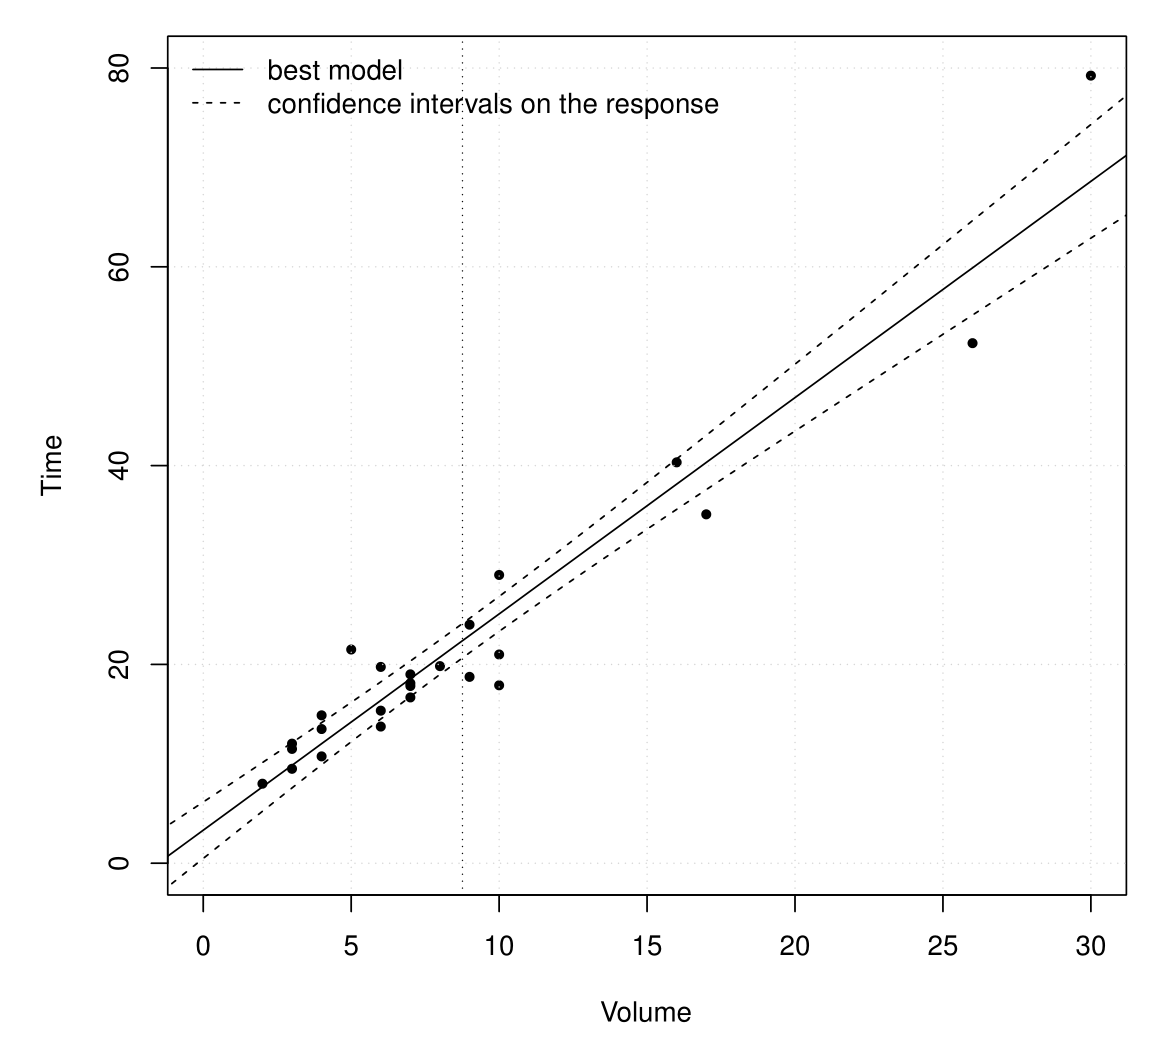
\includegraphics[width=0.5\linewidth]{img/confidence_interval_response_vending_machines}
	\caption{Confidence intervals on the response on the vending machines example}
	\label{fig:confidenceintervalresponsevendingmachines}
\end{figure}

\subsubsection{Prediction Intervals}
Assuming that $x_0$ is the value of the explanatory variable of interest, then $\hat{y}_0 = \beta_0 + \beta_1 x_0$ is the point estimate of the new value of the response $y_0$. The goal is now to find a prediction interval for a future observation, considering the randomness of that observation as well.

\paragraph{Variance} Both random variables $y_0$ and $\hat{y}_0$ are normally distributed, and the expected value of $y_0 - \hat{y}_0$ is thus $0$. The two variables are independent as $y_0$ only depends on the future observation and $\hat{y}_0$ only on the past observations. If two random variables $X$ and $Y$ are uncorrelated then
\begin{equation*}
	\Var{X - Y} = \Var{X} + \Var{Y} + 2\underbrace{\Cov{X-Y}}_0
\end{equation*}
Therefore for the two random variables $y_0$ and $\hat{y}_0$
\begin{align*}
	\Var{y_0 - \hat{y}_0} &= \Var{y_0} + \Var{\hat{y}_0}\\
	&= \sigma^2 + \sigma^2\left(\frac{1}{n} + \frac{(x_0 - \samplemean{x})^2}{S_{xx}}\right)
\end{align*}

\begin{figure}[H]
	\centering
	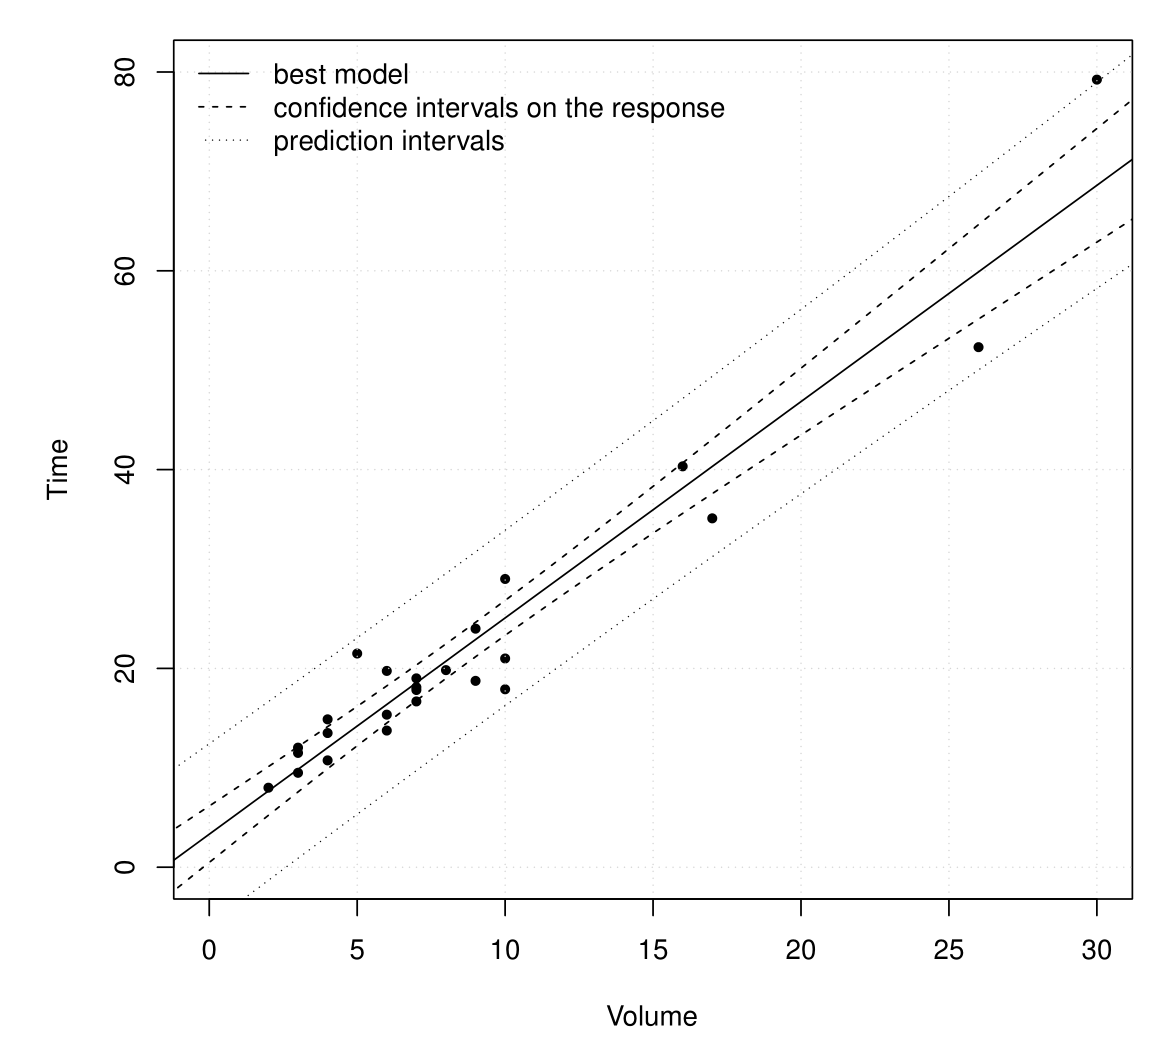
\includegraphics[width=0.5\linewidth]{img/confidence_interval_response_prediction_interval_vending_machines}
	\caption{Prediction and confidence intervals of the vending machines example}
	\label{fig:confidenceintervalresponsepredictionintervalvendingmachines}
\end{figure}

\begin{minted}[
	breaklines=true,
	fontsize=\footnotesize,
	linenos=true,
	stepnumber=5,
	showtabs=true,
	tabsize=4,
	tab=\dotfill
	]{R}
mod <- lm(Time ~ Volume, data)
data.new <- data.frame(Volume=seq(-10, 40, length=101))
Time.Conf <- predict(mod, newdata=data.new, interval="confidence", level=0.95)
Time.Pred <- predict(mod, newdata=data.new, interval="prediction", level=0.95)
#   scatter diagram: Time versus Volume with confidence intervals on the response and prediction intervals
plot(Time ~ Volume, data, pch=20, xlim=c(0,30), ylim=c(0,80), main="Time ~ Volume, best model, CIs on the response, PIs")
grid()
#   add best model
lines(data.new$Volume, Time.Pred[,"fit"], lty=1)
#   add confidence intervals on the response
lines(data.new$Volume, Time.Conf[,"lwr"], lty=2)
lines(data.new$Volume, Time.Conf[,"upr"], lty=2)
#   add prediction intervals
lines(data.new$Volume, Time.Pred[,"lwr"], lty=3)
lines(data.new$Volume, Time.Pred[,"upr"], lty=3)
#   add legend
legend("topleft", legend=c("best model", "confidence intervals on the response", "prediction intervals"), lty=c(1,2,3), bty="n")
\end{minted}

\subsection{Residual Analysis}
\begin{equation*}
	y = \beta_0 + \beta_1 x + \varepsilon
\end{equation*}
Model assumptions
\begin{itemize}
	\item Relationship between response y and regressors x is linear
	\item Error $\varepsilon$ has mean $0$
	\item Error $\varepsilon$ has constant variance $\sigma^2$
	\item Errors are uncorrelated
	\item Errors are normally distributed
\end{itemize}
The problem is that departures from these underlying assumptions are not detectable through the $t$-statistic or the coefficient of determination $R^2$. Thus, the residuals should be investigated, as violated assumptions in the errors should be visible there. The residuals $r_i$ are estimators of the random errors.
\begin{equation*}
	r_i = y_i - \hat{y}_i \quad\forall i\in\{1,\dots,n\}
\end{equation*}
Standardised residuals
\begin{equation*}
	\tilde{r}_{\text{std}, i} = \frac{r_i}{\hat{\sigma} \cdot \sqrt{1-\left(\frac{1}{n} + \frac{(x_i - \samplemean{x})^2}{S_{xx}}\right)}}
\end{equation*}
where $\hat{\sigma}$ is estimated from the data. The goal behind residual analysis is less about justification and more about developing a better model from possible deviations.

\paragraph{Exploratory data analysis}
\begin{itemize}
	\item Improve models based on data
	\item Useful methods for designing appropriate models
	\item Mathematical statements, optimality of statistical methods or statistical significance are less important
\end{itemize}

\subsubsection{Coefficient of Determination $R^2$}
The coefficient of determination quantifies the goodness of the fit of the model
\begin{align*}
	R^2 &= \frac{SS_\text{fit}}{S_{yy}}\\
	\intertext{where}
	SS_\text{fit} &= \sum_{i=1}^{n} (\hat{y}_1 - \samplemean{\hat{y}})^2\\
	&= \sum_{i=1}^{n} \left( (\hat{\beta}_0 + \hat{\beta}_1 x_i) - (\hat{\beta}_0 + \hat{\beta}_1 \samplemean{x}) \right)^2\\
	&= \hat{\beta}_1^2 \cdot \sum_{i=1}^{n} (x_i - \samplemean{x})^2\\
	&= \hat{\beta}_1^2 S_{xx}\\
	S_{yy} &= \sum_{i=1}^{n} (y_i - \samplemean{y})^2
\end{align*}
Therefore, the coefficient of determination is
\begin{equation*}
	R^2 = \hat{\beta}_1^2 \frac{S_{xx}}{S_{yy}}
\end{equation*}
leveraging the fact that $\hat{\beta}_1 = \frac{S_{xy}}{S_xx}$ obtains
\begin{align*}
	R^2 &= \frac{S_{xy}^2}{S_{xx}S_{yy}}\\
	&= \Cor{x,y}^2\\
	&= \frac{\left(\sum_{i=1}^{n} (x_i - \samplemean{x})(y_i - \samplemean{y}) \right)^2}{\sum_{i=1}^{n}(x_i - \samplemean{x})^2 \sum_{i=1}^{n}(y_i - \samplemean{y})^2}
\end{align*}
Thus, $R^2$ is the squared correlation between the explanatory variable $x$ and the response $y$.

In the case of multiple models the coefficient of determination is the squared correlation between the response variable $y$ and the fitted values $\hat{y}$
\begin{equation*}
	R^2 = \Cor{y,\hat{y}}^2 = \frac{S_{y\hat{y}}^2}{S_{yy}S_{\hat{y}\hat{y}}}
\end{equation*}
The interpretation being that this measures the linear relationship between response variable and the fit.

\subsubsection{Diagnostic Tools}
\label{sssec:DiagnosticPlots}
\paragraph{Tukey-Anscombe Plot}
Most powerful and indispensable tool of any residual analysis. It plots the residuals $r_i$ against the fitted values $\hat{y}_i$
\begin{figure}[H]
	\centering
	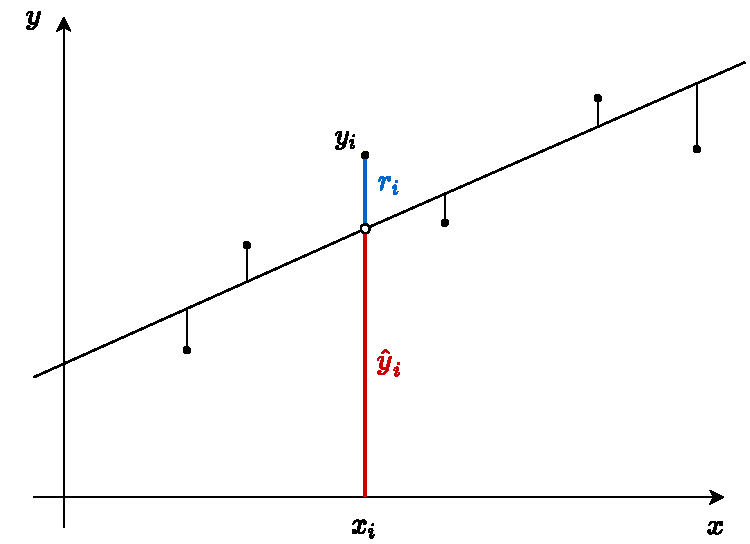
\includegraphics[width=0.5\linewidth]{img/TukeyAnscombe.pdf}
	\caption{Visual representation of the residuals $r_i = y_i - \hat{y}_i$}
\end{figure}
The Tukey-Anscombe plot checks the second model assumption that errors have mean zero, which means that the residuals in any interval of the plot should vary randomly around the horizontal line at zero.
Smooth the residuals using LOESS\footnote{locally estimated scatterplot smoothing} and inspect if the smoothed line varies around the horizontal at zero. Compare with bootstrapped sample if the smoothed residuals lie inside stochastic fluctuations.

\begin{figure}[H]
	\centering
	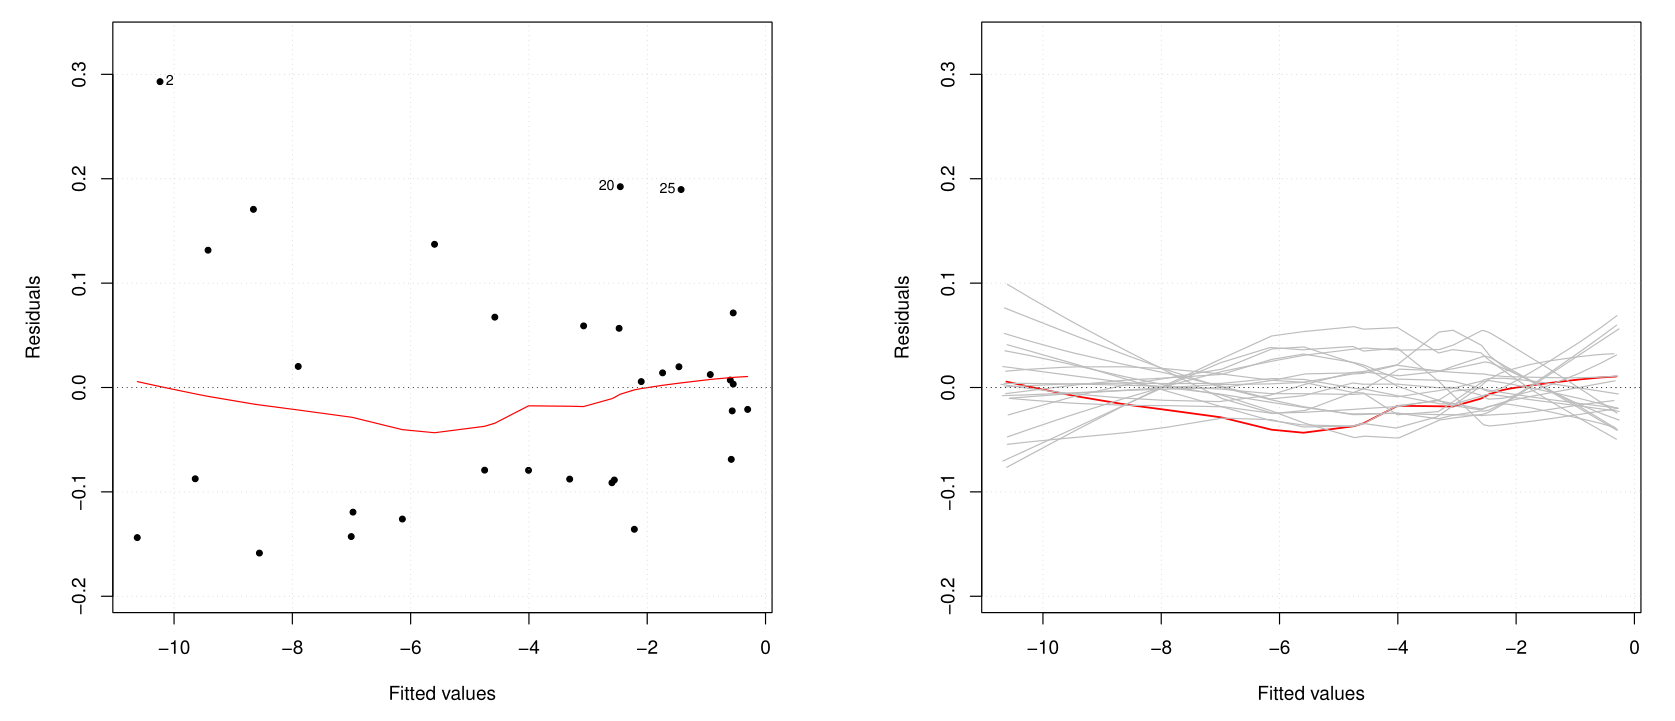
\includegraphics[width=0.8\linewidth]{img/tukey_anscombe_plot}
	\caption{Smoothed residual and bootstrapped residuals}
	\label{fig:tukeyanscombeplot}
\end{figure}


\paragraph{Scale-Location Plot}
Is used to check the third model assumption that errors have equal variance. The square-root of the absolute, standardised residuals $\sqrt{\tilde{r}_{\text{std},i}}$ are plotted against the fitted values of $\hat{y}_i$. If the smoothed curve of the square-root of the absolute, standardised residuals is approximately horizontal, the assumption of equal variance of the errors is not violated.

\begin{figure}[H]
	\centering
	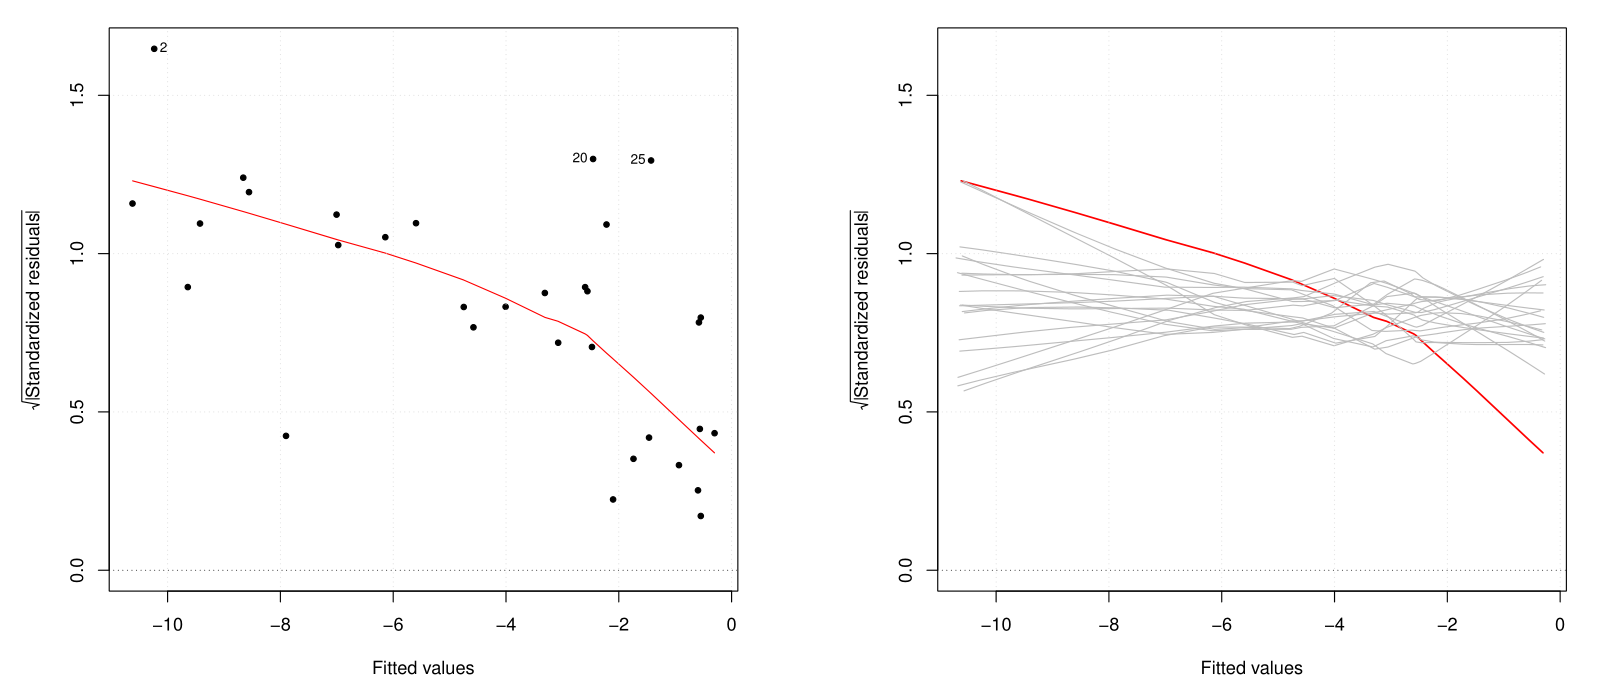
\includegraphics[width=0.8\linewidth]{img/scale_location_plot}
	\caption{Scale-Location plot with smoothed residuals and bootstrapped residuals}
	\label{fig:scalelocationplot}
\end{figure}


\paragraph{Normal Q-Q Plot}
The normal q-q plot is used to test the fifth model assumption that errors are normally distributed. The quantiles of the empirical distribution of the standardised residuals $\tilde{r}_{\text{std},i}$ are plotted against the quantiles of the normal distribution. If the points in the q-q plot scatter around a straight line, then the assumption that errors are normally distribution holds.

\begin{figure}[H]
	\centering
	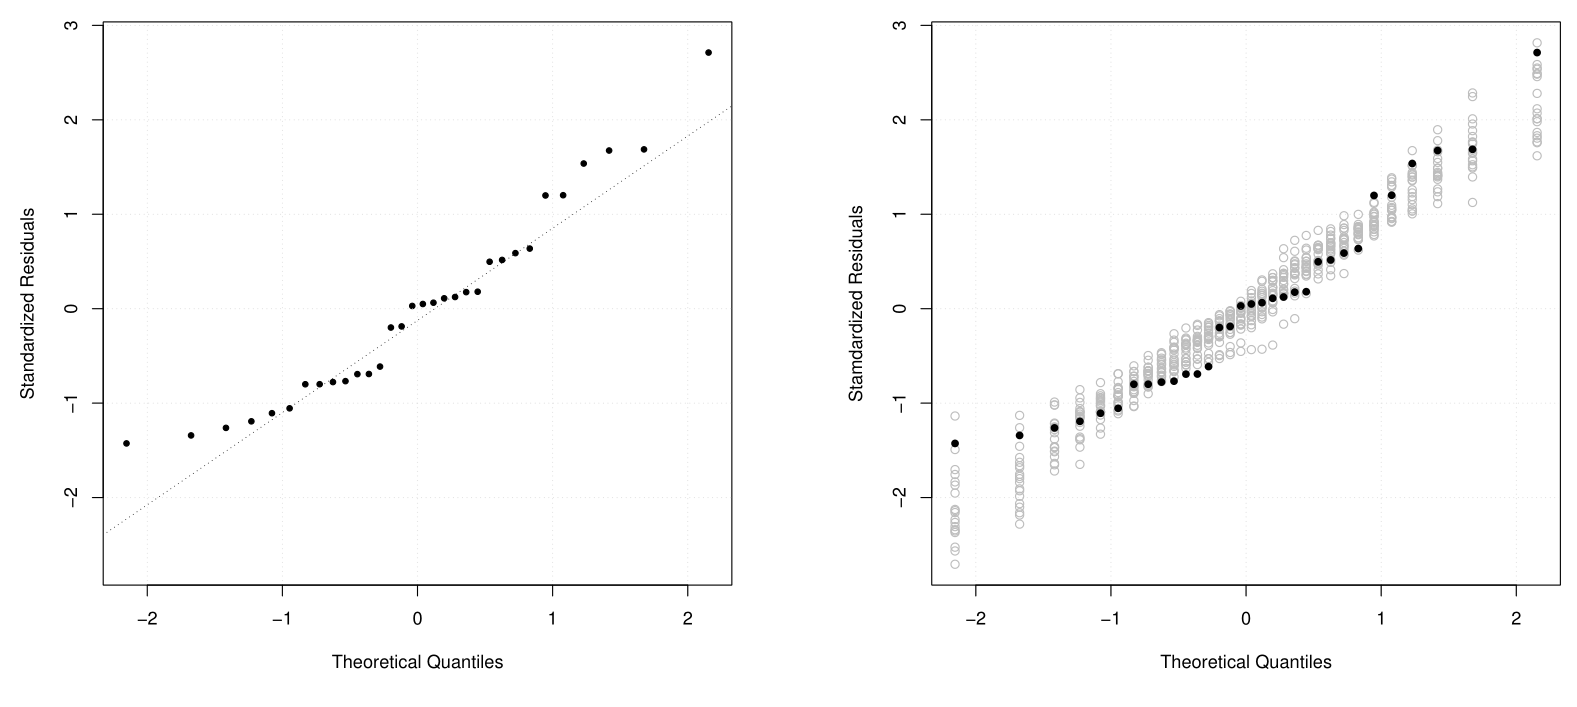
\includegraphics[width=0.8\linewidth]{img/q-q_plot}
	\caption{Q-Q plot and one with simulated residuals}
	\label{fig:q-qplot}
\end{figure}

\subsection{Treatment of Model Violations}
Through the use of diagnostic tools \textit{characterise inadequacies} of the model, \textit{investigate their cause} and \textit{eliminate problems}. Frequent violations are
\begin{itemize}
	\item Non-constant variance of random errors
	\item Outliers
	\item Heavy-tailed distributions
\end{itemize}

\subsubsection{Tukey's First Aid Transformations}
\begin{itemize}
	\item \textbf{Logarithmic} for continuous positive variables\\
	\begin{equation*}
		z \longmapsto \log(z)
	\end{equation*}
	\item \textbf{Square-root} for continuous and discrete positive variables\\
	\begin{equation*}
		z \longmapsto \sqrt{z}
	\end{equation*}
	\item \textbf{Arcsine} for proportions\\
	\begin{equation*}
		z \longmapsto \arcsin(\sqrt{z})
	\end{equation*}
	\item \textbf{Logit} for proportions\\
	\begin{equation*}
		z \longmapsto \log\left(\frac{z+{\color{gray}\varepsilon_1}}{1+{\color{gray}\varepsilon_2}-z}\right)
	\end{equation*}
\end{itemize}

\subsubsection{Additive and Multiplicative Error Terms}
\textbf{log-log} Transformation of the explanatory and response variable
\begin{align*}
	\tilde{x} &= \log(x)\\
	\tilde{y} &= \log(y)
\end{align*}
The additive error $\varepsilon$
\begin{align*}
	\tilde{y} = \beta_0 + \beta_1 \tilde{x} + \varepsilon\\
	\log(y) = \beta_0 + \beta_1 \log(x) + \varepsilon
\end{align*}
is transformed to a multiplicative model
\begin{equation*}
	y = e^{\beta_0 + \beta_1 \log(x) + \varepsilon} = e^{\beta_0}\cdot e^{\beta_1\log(x)}\cdot e^{\varepsilon}  =e^{\beta_0}\cdot x^{\beta_1}\cdot e^{\varepsilon}
\end{equation*}
with the multiplicative random error $e^\varepsilon$.

\subsection{Correlation Plots}
% TODO Write Correlation Plots and assumption of uncorrelated errors

\subsection{Multiple Linear Regression}
\textbf{Multiple Linear Regression Model}
\begin{equation*}
	y = \beta_0 + \beta_1\cdot x_1 + \beta_2\cdot x_2 + \dots + \beta_m\cdot x_m + \varepsilon
\end{equation*}
To find the least-squares estimators $\beta_0,\beta_1,\dots,\beta_m$, for each measurement $X_i$
\begin{equation*}
	y_i = \beta_0 + \sum_{k=1}^{m}\beta_k x_{ik} + \varepsilon_i
\end{equation*}
with $i\in\{1,2,\dots,n\}$.

This is much easier done with linear algebra
\begin{equation*}
	\bm{y} = \begin{pmatrix}
		y_1\\y_2\\\vdots\\y_n
	\end{pmatrix} \quad\text{and}\quad \bm{X} = \begin{pmatrix}
		1 & x_{11} & x_{12} & \cdots & x_{1m}\\
		1 & x_{21} & x_{22} & \cdots & x_{2m}\\
		\vdots & \vdots & \vdots & \ddots & \vdots\\
		1 & x_{n1} & x_{n2} & \cdots & x_{nm}
	\end{pmatrix}
\end{equation*}
\begin{equation*}
	\bm{\varepsilon} = \begin{pmatrix}
		\varepsilon_1\\\varepsilon_2\\\vdots\\\varepsilon_n
	\end{pmatrix} \quad\text{and}\quad \bm{\beta} = \begin{pmatrix}
		\beta_0\\\beta_1\\\beta_2\\\vdots\\\beta_m
	\end{pmatrix}
\end{equation*}
and thus the model becomes
\begin{equation*}
	\bm{y} = \bm{X\beta + \varepsilon}
\end{equation*}
The goal of the least squares estimator is the same as in the simple linear regression, which is to minimise the residual sum of squares
\begin{align*}
	S(\bm{\beta}) &= \sum_{i=1}^{n}\varepsilon_i^2\\
	&= \varepsilon^t\varepsilon\\
	&= (\bm{y-X\beta})^t (\bm{y-X\beta})\\
	&= \bm{y}^t\bm{y} - 2\bm{\beta}^t\bm{X}^t\bm{y} + \bm{\beta}^t\bm{X}^t\bm{X\beta}
\end{align*}
The least-squares estimators $\hat{\bm{\beta}}$ must satisfy the stationary condition $\frac{\partial S}{\partial \bm{\beta}} = 0$
\begin{equation*}
	\frac{\partial S}{\partial \bm{\beta}}(\hat{\bm{\beta}}) = - 2\bm{X}^t\bm{y} + 2\bm{X}^t\bm{X\beta}
\end{equation*}
Least-squares normal equations
\begin{align*}
	\bm{X}^t\bm{\beta} &= \bm{X}^t\bm{X}\hat{\bm{\beta}}\\
	\hat{\bm{\beta}} &= (\bm{X}^t\bm{X})^{-1}\bm{X}^t\bm{y}\\
	\intertext{Fitted values}
	\hat{\bm{y}} &= \bm{X}\hat{\bm{\beta}}\\
	&= \bm{X}(\bm{X}^t\bm{X})^{-1}\bm{X}^t\bm{y}\\
	&= \bm{H}\bm{y}
\end{align*}
The hat matrix $\bm{H}$ maps the observed values $\bm{y}$ to the fitted values $\hat{\bm{y}}$. It's called that way as it puts $\bm{y}$ a hat on.

The residuals can be calculated the following way
\begin{align*}
	\bm{e} &= \bm{y} - \hat{\bm{y}}\\
	&= \bm{y} - \bm{H}\bm{y}\\
	&= (\bm{I} - \bm{H}) \bm{y}
\end{align*}
where $\bm{I}$ is the $n\times n$ identity matrix.

\subsubsection{Significance Tests of Regression Coefficients}
The assumption is that the least-squares estimators $\hat{\bm{\beta}}$ are normally distributed.
\begin{equation*}
	\ev{\hat{\bm{\beta}}} = \bm{\beta}\quad\text{and}\quad\Cov{\hat{\bm{\beta}}} = \sigma^2(\bm{X}^t\bm{X})^{-1}
\end{equation*}
The null hypothesis $H_0$ is that
\begin{equation*}
	\beta_k = \beta_{k,0}
\end{equation*}
and the test statistic
\begin{equation*}
	T_k = \frac{\hat{\beta}_k - \beta_{k,0}}{\se{\hat{\beta}_k}}\quad\text{with}\quad\se{\hat{\beta}_k} = \hat{\sigma}\sqrt{\left((\bm{X}^t\bm{X})^{-1}\right)_{kk}}
\end{equation*}
with the residual sum of squares $\hat{\sigma}^2 = \frac{\bm{e}^t\bm{e}}{n-(m+1)}$ and $T_k$ following a Student's $t$-distribution with $n-(m+1)$ degrees if freedom.

As a conclusion, if the null hypothesis $H_0$ is not rejected, then the regressor $x_k$ can be omitted from the model. The $100\cdot(1-\alpha)$ percent confidence interval on $\beta_k$ is
\begin{equation*}
	\hat{\beta}_k - t_{\frac{\alpha}{2},n-(m+1)}\cdot\se{\hat{\beta}_k} \leq \beta_k \leq \hat{\beta}_k + t_{1 - \frac{\alpha}{2},n-(m+1)}\cdot\se{\hat{\beta}_k}
\end{equation*}
where $\se{\hat{\beta}_k} = \hat{\sigma}\sqrt{\left((\bm{X}^t\bm{X})^{-1}\right)_{kk}}$.

\subsubsection{Confidence Interval of the Response}
The estimated value $\hat{y}_0$ is an unbiased, normally distributed estimator
\begin{align*}
	\hat{y}_0 &= \hat{\beta}_0 + \hat{\beta}_1 x_{0,1} + \hat{\beta}_2 x_{0,2} + \dots + \hat{\beta}_m x_{0,m}\\
	&=\bm{x}_0^t \hat{\bm{\beta}}\\
	\Var{\hat{y}_0} = \sigma^2 \bm{x}_0^t(\bm{X}^t\bm{X})^{-1}\bm{x}_0
\end{align*}
with a confidence interval on the response
\begin{equation*}
	\hat{y}_0 - t_{\frac{\alpha}{2},n-(m+1)}\cdot\se{\hat{y}_0} \leq \beta_k \leq \hat{y}_0 + t_{1 - \frac{\alpha}{2},n-(m+1)}\cdot\se{\hat{y}_0}
\end{equation*}
with the standard error being
\begin{equation*}
	\se{\hat{y}_0} = \hat{\sigma}\sqrt{\bm{x}_0^t(\bm{X}^t\bm{X})^{-1}\bm{x}_0}
\end{equation*}

% TODO Confidence Interval Response

% TODO Prediction Interval

% TODO Coefficient of Determination

\subsection{Diversity of Modelling Parameters}

\subsubsection{Polynomial Regression}
When there is a curved relationship, low-order polynomial functions can be used. Example model with polynomial of degree two
\begin{equation*}
	y = \beta_0 + \beta_1 x + \beta_2 x^2 + \varepsilon
\end{equation*}
This is a simple linear regression with a quadratic function.

\subsubsection{Non-linear Functions and Linear Regression}
Transforming the variables to get better fitting results may introduce non-linear relationships.
\begin{align*}
	y = \frac{1}{a+be^{-x}} &\longrightarrow \frac{1}{y} = a + be^{-x}\\
	y = \frac{ax}{b+x} &\longleftrightarrow \frac{1}{z} = \frac{1}{a} + \frac{b}{a}\frac{1}{x}\\
	y = ax^b &\longrightarrow \ln{(y)} = \ln{(a)} + b\ln{(x)}
\end{align*}
All these models are linear models, however this is not always possible. Non-linear models can be fitted with the package \mintinline{R}{nls}.

\subsubsection{Binary Explanatory Variables}
% TODO Binary Explanatory Variables

\subsubsection{Factor Variables}
A factor variable is a discrete variable with $s$ levels $\{l_1, l_2,\dots,l_s\}$. These can be transformed to binary dummy variables $x_k^{(j)} = (x_{k,1}^{(j)}, x_{k,2}^{(j)}, \dots, x_{k,n}^{(j)})$ with
\begin{equation*}
	x_k^{(j)} \left\{
		\begin{matrix}
			1 & \text{if $i$th observation $x_{k,i}$ is equal to $j$th level $l_j$}\\
			0 & \text{otherwise}
		\end{matrix}
	\right.
\end{equation*}
The regression model then becomes
\begin{equation*}
	y = \beta_0 + \beta_1x_1 + \dots + (\beta_{k,2}x_k^{(2)} + \dots + \beta_{k,s}x_k^{(s)}) + \dots + \beta_m x_m + \varepsilon
\end{equation*}
To force the uniqueness of the optimisation problem the first level $\beta_{k,1}$ has to be zero, so that there are only $s-1$ dummy variables for a factor variable with $s$ levels.

\subsubsection{Comparison of Multiple Regression Models with an \textit{F}-Test}
% TODO Write Comparison of Models using F-Test

\subsubsection{Modelling of Two Straight Lines}
\begin{figure}[H]
	\centering
	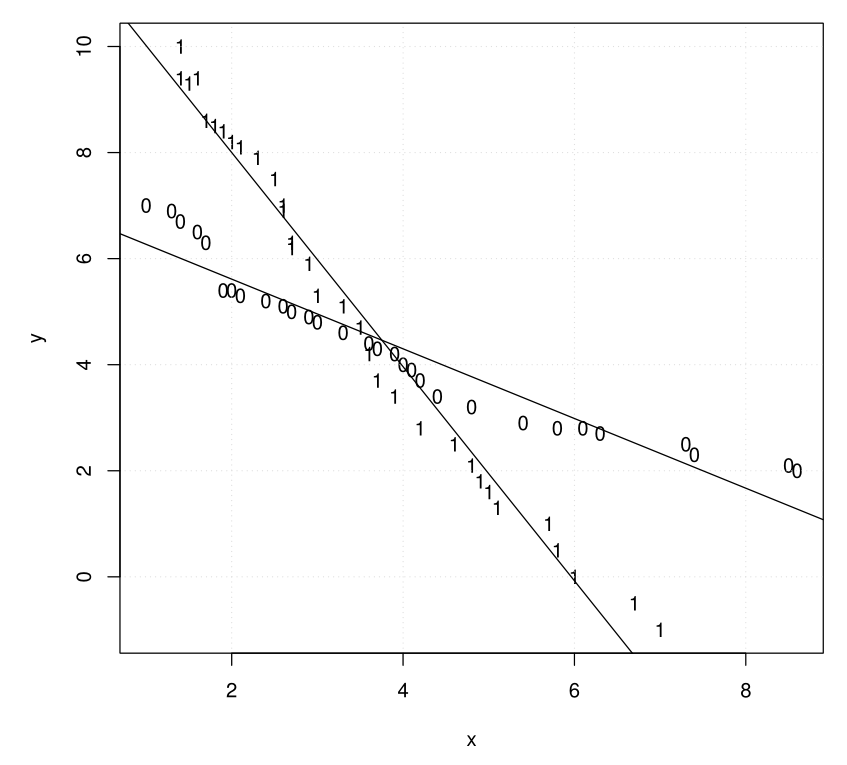
\includegraphics[width=0.4\linewidth]{img/two_straigt_lines}
	\caption{Straight regression lines through data with two groups}
	\label{fig:twostraigtlines}
\end{figure}
To model this relationship a multiple regression model with a factor variable which indicates group membership must be used
\begin{equation*}
	g_i = \left\{
	\begin{matrix}
		0 & \text{observation $i$ belongs to the first line}\\
		1 & \text{observation $i$ belongs to the second line}
	\end{matrix}
	\right.
\end{equation*}
% TODO Finish Group Models

\subsection{Sensitivity and Robustness}
In multiple linear regression too many dimensions are involved and the regression model cannot be properly visualised. However, the diagnostic plots introduced in \ref{sssec:DiagnosticPlots} can still be used.
\begin{enumerate}
	\item Analyse and compare with bootstrap simulations
	\begin{itemize}
		\item Tukey-Anscombe plot
		\item scale-location plot
		\item q-q plot
		\item residuals versus leverage
		\item time dependencies in the residuals (plot residuals against index)
	\end{itemize}
	\item Draw conclusions, analyse biggest discrepancies and remedies
\end{enumerate}
\begin{figure}[H]
	\centering
	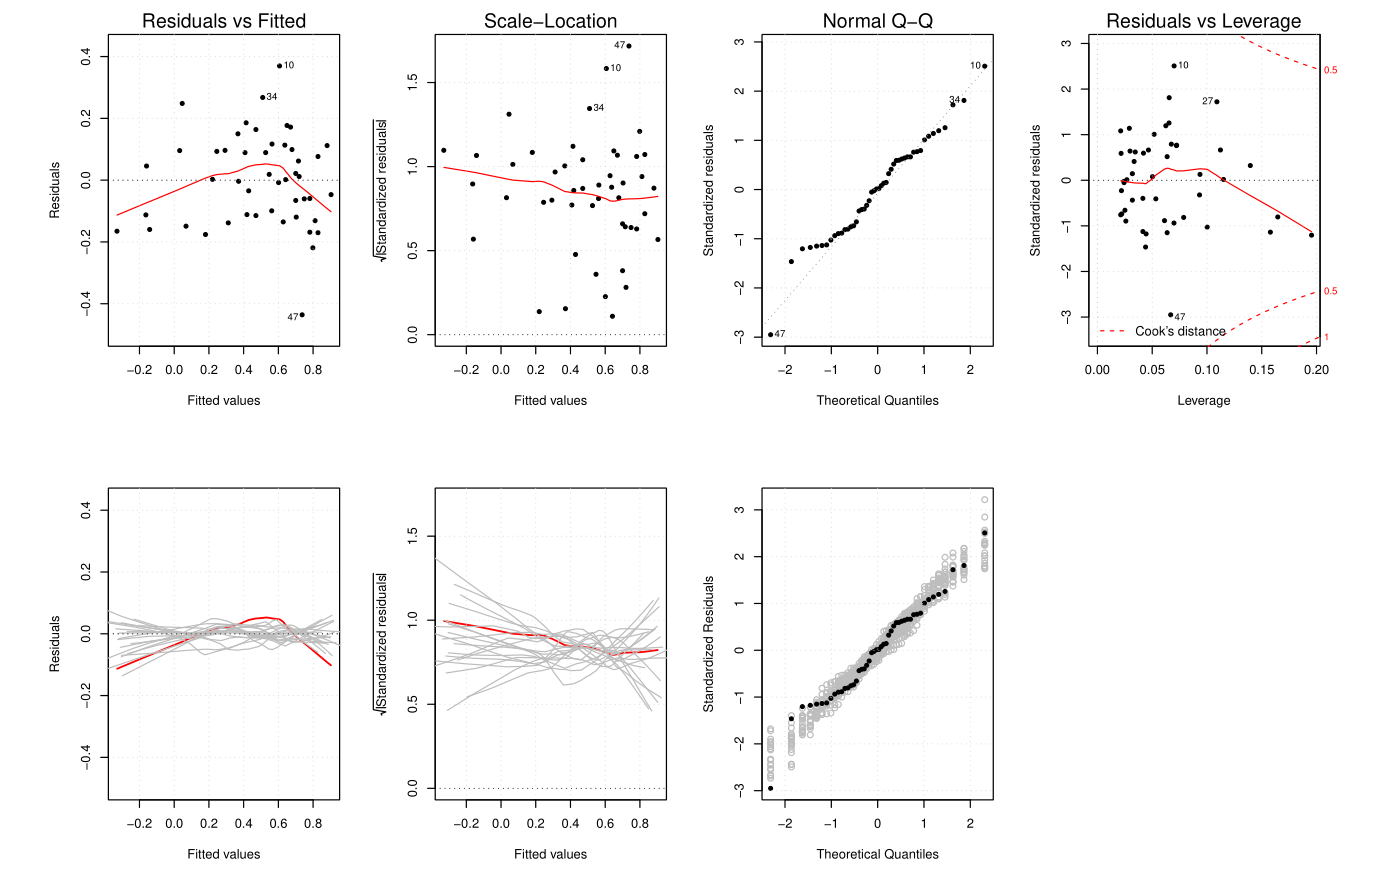
\includegraphics[width=0.8\linewidth]{img/diagnostic_plots_blasting}
	\caption{Diagnostic plots for the multi-dimensional model of the \texttt{Blasting} dataset}
	\label{fig:diagnosticplotsblasting}
\end{figure}
Even though the Tukey-Anscombe diagram shows deviations in the $\N{0,\sigma^2}$ but in multiple regression it's not longer clear which explanatory variable causes deficits.

Thus, a new diagram is introduced which plots the residuals $e$ of each explanatory variable $x_1,\dots,x_k\dots,x_m$ against $x_k$. In this plot the assumption can again be checked.
\begin{figure}[H]
	\centering
	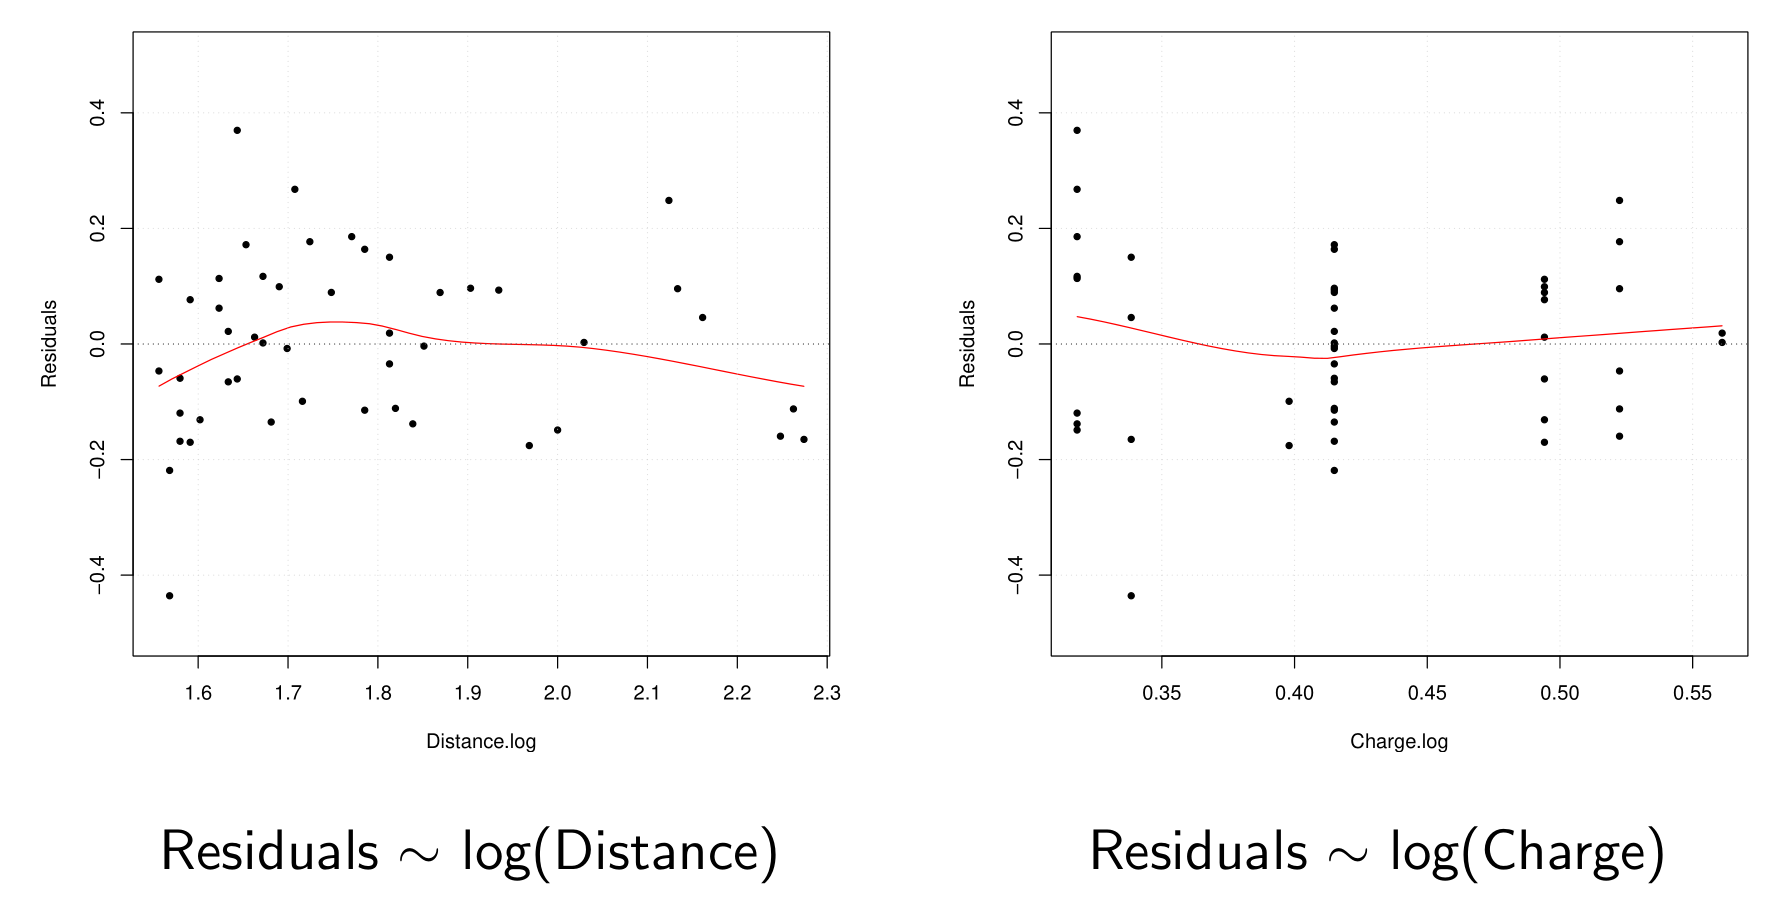
\includegraphics[width=0.7\linewidth]{img/diagnostic_plots_residuals_explanatory}
	\caption{Plots of residuals against their explanatory variable}
	\label{fig:diagnosticplotsresidualsexplanatory}
\end{figure}

\subsubsection{Influential Observations}
An outlier can be identified by investigating the influence of said data point. This is done by removing the observation, repeating the analysis and measuring the change.\footnote{\href{https://online.stat.psu.edu/stat501/lesson/11/11.1}{PennState Eberly College of Statistics - Distinction Between Outliers \& High Leverage Observations}}

\vspace{1em}
\noindent
\textbf{Cook's distance measure}
\begin{equation*}
	d_i  = \frac{(\hat{\bm{y}}_{\\i} - \hat{\bm{y}})^T(\hat{\bm{y}}_{/i} - \hat{\bm{y}})}{p\hat{\sigma}^2}
\end{equation*}
where $\hat{\bm{y}}=\bm{X}\hat{\bm{\beta}}$ is the $n\times1$ vector of the fitted values, $\hat{\bm{y}}_{\\i}=\bm{X}\hat{\bm{\beta}}_{\\i}$ the $n\times1$ vector of fitted values without observation $i$, and $p$ the number of estimated parameters.

Fortunately the analysis does not have to be repeated $n$ times
\begin{equation*}
	d_i = \frac{e_i^2}{p\hat{\sigma}^2}\frac{h_{ii}}{(1-h_{ii})^2} = \frac{\tilde{e}_{\text{std}, i}^2}{p}\frac{h_{ii}}{(1-h_{ii})^2}
\end{equation*}
where $e_i$ is the $i$th residual and $\tilde{e}_{\text{std},i}$ the standardised residual. The leverages satsify
\begin{equation*}
	0\leq h_{ii}\leq 1\qquad\text{and}\qquad \bar{h} = \frac{p}{n}
\end{equation*}

\paragraph{Interpretation of Leverages}
If a response $y_i$ is changed by the amount $\Delta_{y_i}$, then $h_{ii}\Delta_{y_i}$ measures the change in the fitted value $\hat{y}_i$. \textit{A large leverage $h_{ii}$ has a big influence on the fitted values}.

The variance of the $i$th residual is 
\begin{equation*}
	\Var{e_i} = (1-h_{ii})\sigma^2
\end{equation*}
\textit{A large leverage $h_{ii}$ reduces the variance of the $i$th residual, and therefore the $i$th observation is close to regression hyper-plane. Leverage is a measure of how far away the explanatory values of an observation are from those of the other observations.}

\paragraph{Identification of Leverage Points}
A good rule of thumb is that observations are dangerous if
\begin{equation*}
	h_{ii} > 2\frac{p}{n}
\end{equation*}

\paragraph{Huber's Classification of Observations} gives a notion of leverage issues
\vspace*{1em}
\begin{tabularx}{\linewidth}{X X}
	\textbf{Leverage} & \textbf{Classification} \\
	\hline
	$h_{ii} < 0.2$ & harmless \\
	$0.2 < h_{ii} < 0.5$ & potentially problematic \\
	$0.5 < h_{ii}$ & should be avoided \\
\end{tabularx}

\paragraph{Identification using Cook's distance measure} with the rule of thumb
\begin{tabularx}{\linewidth}{c X}
	\textbf{Cook's distance} & \textbf{Classification of $i$th observation} \\
	\hline
	$d_i \leq 1$ & harmless \\
	$1 < d_i$ & problematic
\end{tabularx}

\begin{figure}[tbh]
	\centering
	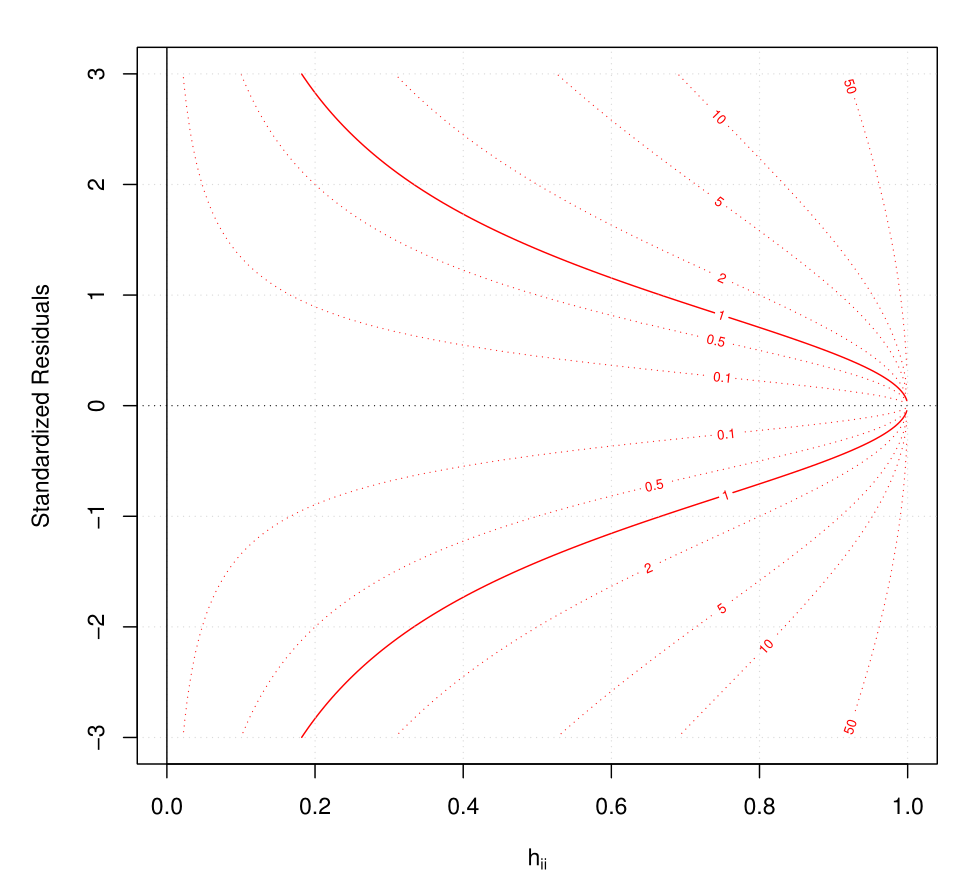
\includegraphics[width=0.6\linewidth]{img/cook_distance_contour_plot}
	\caption{Contour plot of Cook's distance measure can be used to quickly identify problematic observations. $d(h, \tilde{e}_{\text{std}}) = \frac{\tilde{e}^2_{\text{std}}}{p}\frac{h}{1-h}$}
	\label{fig:cookdistancecontourplot}
\end{figure}



% TODO Finish Sensitivity and Robustness

\subsection{Variable Selection and Modelling}
There are two approaches to modelling, with \textbf{mechanistic models} where the functional relationships are known and the model is used for parameter, confidence and prediction interval estimation. The others are \textbf{empirical models} where the influence of explanatory variables on the response are unknown, and the models are used to investigate the relationship between response and explanatory variables.

Which  explanatory variables should be used in which form in the regression model? With a regression model the explanatory variables $x_1,\dots,x_m$ in
\begin{equation*}
	y = \beta_0 + \beta_1 x_1 + \beta_2 x_2 + \dots + \beta_m x_m + \varepsilon
\end{equation*}
can be transformed into observations $u_k$ like
\begin{equation*}
	x_k = log(u_k) \quad\text{and}\quad x_k = \frac{1}{u_k}
\end{equation*}
or by combination of several observations $u_k, u_l$ like
\begin{equation*}
	x_j = u_k\cdot u_l\quad\text{or}\quad x_j = \frac{u_k + u_l}{2}
\end{equation*}
The same is true for the response $y$.

\subsubsection{Model Selection Methods}
\begin{quote}
	\textquotedblleft Plurality must never be posited without necessity\textquotedblright\\
	\hspace*{2em} -William of Ockham
\end{quote}
The idea for better generalising model is to measure model accuracy and penalise model complexity. This leads to a trade-off between model complexity and accuracy.

\paragraph{Adjusted $R$-Squared}
\begin{equation*}
	R_{\text{adj}}^2 = 1 - \frac{n-1}{n-p}(1-R^2) = R^2 - \frac{p-1}{n-p}(1-R^2)
\end{equation*}
with $R^2$ being the coefficient of determination, $n$ being the number of observations and $p=m+1$ being the number of parameters in the model. $R_{\text{adj}}^2\leq R^2$ and $R_{\text{adj}}^2$ gets smaller with increasing number of parameters $p$.

\paragraph{Akaike Information Criterion}
\begin{equation*}
	\text{AIC} = n\ln\left(\frac{1}{n}\sum_{i=1}^{n}e_i^2\right) + 2\tilde{p} + \text{constant}
\end{equation*}
with $n$ being the number of observations, $e_1,\dots,e_n$ being the $n$ residuals and $\tilde{p}$ the number of model parameter with $\sigma$ included.

The Akaike information criterion is the most generalisable criterion and it is also used in time series analysis.

\paragraph{Mallow's $C_p$ Statistic}
\begin{equation*}
	C_p = \frac{\text{SS}_{E}}{\hat{\sigma}_{p^*}^2} + 2p - n = (n-p)\left(\frac{\hat{\sigma}_{p}^2}{\hat{\sigma}_{p^*}^2}\right) + p
\end{equation*}
with $n$ being the number of operations, $\text{SS}_E$ the sum of squares of the errors, $\hat{\sigma}_{p}^2 = \frac{\text{SS}_E}{n-p}$ the estimator of $\sigma^2$ of the model with $p$ parameters, and $\hat{\sigma}_{p^*}^2$ the estimator of $\sigma^2$ of the full model with $p^*$ parameters.

Mallow’s $C_p$ statistic minimises the prediction error.

\paragraph{Forward Selection}
\begin{enumerate}
	\item In the first step choose the trivial model with an intercept only
	\begin{equation*}
		y=\beta_0 + \varepsilon
	\end{equation*}
	\mintinline{R}{formula = y ~ 1}
	\item In the following steps, the explanatory variable that leads to the largest improvement of the selected model selection criteria is added in the model.
	\item Iterate until no improvement is possible by adding another explanatory variable.
\end{enumerate}

\paragraph{Backward Elimination}
\begin{enumerate}
	\item In the first step choose the full model with all possible explanatory variables
	\begin{equation*}
		y=\beta_0 + \beta_1 x_1 + \beta_2 x_2 + \dots + \beta_m x_m + \varepsilon
	\end{equation*}
	\mintinline{R}{formula = y ~ 1}
	\item In the following steps, the explanatory variable that leads to the largest improvement of the selected model selection criteria is added in the model.
	\item Iterate until no improvement is possible by adding another explanatory variable.
\end{enumerate}

\paragraph{Forward Selection}
Combination of forward selection and backward elimination
\begin{enumerate}
	\item In the first step choose any model
	\item In the following steps examine whether eliminating or adding an explanatory variable improves the selected model selection criteria. The action that leads to the largest improvement is carried out.
	\item Iterate until no improvement is possible.
\end{enumerate}

\subsubsection{Collinearity}
High correlation coefficients between explanatory variables are allowed in the estimation procedure, but this makes interpretation of the estimated coefficients difficult.
\begin{definition}
	\textbf{Collinearity} is when an offset $\gamma_0$ and coefficients $\gamma_1,\dots,\gamma_{k-1},\gamma_{k+1},\dots,\gamma_m$ exist, such that
	\begin{equation}
		x_k\approx \gamma_0 + \sum_{j,j\neq k}^{m} \gamma_j x_j
		\label{eq:linear_multiple_regression_model}
	\end{equation}
\end{definition}
 If this relation is exact then the least-squares estimator is not uniquely defined and software implementations may have problems.

\paragraph{Measure for Collinearity} with the linear multiple regression model (eq. \ref{eq:linear_multiple_regression_model}) and a coefficient of determination $R_k^2$ for each $x_1,\dots,x_m$.

Then the \textbf{variance inflation factor} of explanatory variable $x_k$ is
\begin{equation*}
	\text{VIF}_k = \frac{1}{1 - R_k^2}
\end{equation*}
This factor is problematic if $\text{VIF} > 5$ (rule of thumb).

\subsubsection{Modelling Strategies}
Humans do modelling not machines!
\begin{itemize}
	\item Automated variable selection depends on chance.\\
	Consider models that are nearly optimal in terms of the selected criteria.
	\item Optimal model do not necessarily have to meet all model requirements.\\
	Residual analysis
	\item Automated variable selection starts with given set of variables.\\
	Transformations and interactions are ignored.
	\item Automated variable selection may provide models and estimated coefficients that contradict first principles.
	\item The concept of a best model may also depend on the purpose.
\end{itemize}
Important points in modelling
\begin{itemize}
	\item \textbf{Residual Analysis}
	\begin{itemize}
		\item Check the assumptions of independence, constant variance, linearity and normal distribution
		\item Identify influential observations and use robust methods as a remedy
	\end{itemize}
	\item \textbf{Transformations}
	\begin{itemize}
		\item Transform the response as well as the explanatory variables
		\item Add interactions
		\item Expand the model with factor variables
	\end{itemize}
	\item \textbf{Variable Selection}\\
	Do not blindly trust automatic variable selection and use your brain!
\end{itemize}

\subsubsection{Overall Modelling Strategy}
\begin{enumerate}
	\item Understanding the problem\\
	Any models already available?
	\item Collection and Processing of data
	\begin{itemize}
		\item Missing values?
		\item Treatment of missing values?
		\item Meaning of null values in variables
		\item First-Aid Transformations of variables
		\item Keep track of data quality
	\end{itemize}
	\item Model fitting, eventually with a robust method
	\item Residual Analysis\\
	If problems are identified, backtrack until problems are remedied
	\item Variable selection and treatment of collinearity
	\item Checking goodness of fit
	\begin{itemize}
		\item Residual analysis with selected models
		\item Match models with first principles
		\item Validate models with data not used in modelling
	\end{itemize}
\end{enumerate}

\subsubsection{Generalisations of Multiple Linear Regression}
\begin{itemize}
	\item \textbf{Non-linear regression}\\
	More complicated functions can be fitted
	\item \textbf{Nonparametric regression}\\
	Less assumptions on the models are made (smoothing)
	\item \textbf{Generalised linear model}\\
	Response variable is allowed to have error distribution models other than normal (Logistic, Poisson and Gamma-regression)
	\item \textbf{Survival analysis}\\
	Censored data (reliability theory, survival and hazard function)
	\item \textbf{Time series analysis}\\
	The errors can be correlated
	\item \textbf{Principal component} and \textbf{partial least squares regression}\\
	More variables than observations: large $p$, small $n$ (chemometrics)
\end{itemize}

\section{Design of Experiments}
\begin{itemize}
	\item[] \textbf{Experiment}
	\item Well defined situation
	\item Analysed variables systematically varied
	\item Background noise under control
	\item[] \textbf{Survey}
	\item Observations in the context of an existing situation
	\item Analysed variables not directly adjustable
	\item Background noise not at all under control
\end{itemize}

\subsection{Terminology and Concepts}
Response variable depends on many explanatory variables
\begin{itemize}
	\item \textbf{Primary variables} are directly connected with the research topic
	\item \textbf{Secondary variables} are also controllable with a reasonable effort
\end{itemize}
Basic idea of an experiment is, that primary and secondary variables can be varied in a prescribed controlled manner.

\begin{figure}[H]
	\centering
	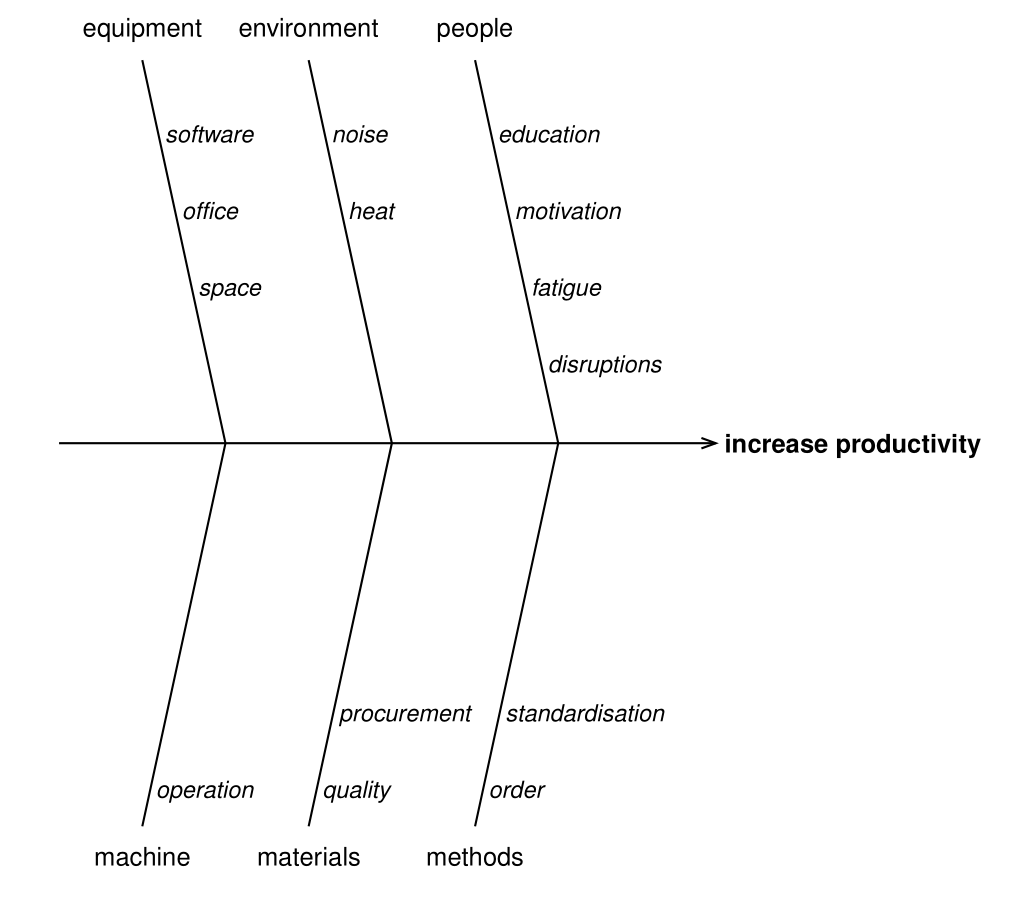
\includegraphics[width=0.6\linewidth]{img/cause_and_effect_diagram}
	\caption{The cause-and-effect diagram is a tool for identifying all influental factors}
	\label{fig:causeandeffectdiagram}
\end{figure}

\subsubsection{Obtaining Precise Primary Variable Estimates}
\begin{itemize}
	\item For continuous variables $x$ choose values $x_i$ without any condition; choosing $x_i$ equally spaced gives good estimates for the slope and chances to detect deviation from linearity; variance of slope is minimal if sum of squares $S_{xx}$ is maximal (choose wider range of $x$-values)
	\item For factor variables, record the same number of $y$-values for each level
	\item For several different variables make an effort to choose them as independent as possible
	\begin{itemize}
		\item For continuous variables choose an orthogonal design
		\item For factors choose a balanced design
	\end{itemize}
\end{itemize}

\subsubsection{Obtaining Precise Secondary Variable Estimates}
\begin{itemize}
	\item[] \textbf{Block designs}\\
	Record additional variables, that is batches, production lot or origin of product
	\item Precision can be increased (if variable is significant)
	\item Interpretability of the results can be simplified
	\item[] \textbf{Randomisation}\\
	Perform experiments in random order
	\item Chronological order as independent as possible from all recorded and unrecorded variables
	\item Prevent influences due to the system of the experimental conditions
	\item Avoid learning effects or aging of a device
\end{itemize}

\subsubsection{Obtaining Precise Response Variable Estimates}
\begin{itemize}
	\item[] \textbf{Replicates}\\
	Multiple measurements with same experimental conditions
	\item Improved accuracy of the statements
	\item Estimate of the variation of the random errors available
	\item Existence of interactions in analysis of variance can be tested
	\item Replicates are not allowed to be measured consecutively, otherwise they are not independent
	\item Randomise replicates despite the increased experimental effort
\end{itemize}
Alternative: Add more explanatory variables, but beware because many studies fail because of too extensive investigations with too few observations.

% TODO Design of Experiments

% TODO 13 Factorial Designs

\subsection{Screening Experiments}
A process is influenced by many factors, but not all of them may be relevant or significant. The idea is thus to experimentally examine the interaction of factors on the response variable by observing the process under different conditions.

\subsubsection{$2^k$ Factorial Design}
The problem is, that the number of experiments rapidly increases to an unrealistically large number as more factors are involved. The solution is to have only a binary level per factor which leads to $2^k$ runs with $k$ factors.
\begin{tabularx}{\linewidth}{c | c c c | c}
	\multicolumn{5}{l}{\textbf{Design Matrix}}\\[0.5em]
	Run & \multicolumn{3}{c|}{Factors} & Letters\\
	& A & B & C & \\
	\hline
	1 & $-1$ & $-1$ & $-1$ & (1) \\
	2 & $+1$ & $-1$ & $-1$ & a   \\
	3 & $-1$ & $+1$ & $-1$ & b   \\
	4 & $+1$ & $+1$ & $-1$ & ab  \\
	5 & $-1$ & $-1$ & $+1$ & c   \\
	6 & $+1$ & $-1$ & $+1$ & ac  \\
	7 & $-1$ & $+1$ & $+1$ & bc  \\
	8 & $+1$ & $+1$ & $+1$ & abc \\
\end{tabularx}
Design matrix in \textbf{Yates standard order}, but runs of the experiment in randomised order.

\paragraph{Estimate main effect} The main effect of a factor is the average response value for all test runs at the high level of the factor minus the average response value for runs at the low level of the factor.

The two factor interaction effect is one-half of the difference between the main effects of one factor calculated at the two levels of the other factor.

\paragraph{Half-Normal Plot} Are used to estimate if effects are significant. If effects are zero then estimates are only noise. Estimated effects are realisations of the same noise. Significant effects show up as outliers. Thus, plot the absolute values of effects versus the quantiles of the normal distribution.
\begin{figure}[H]
	\centering
	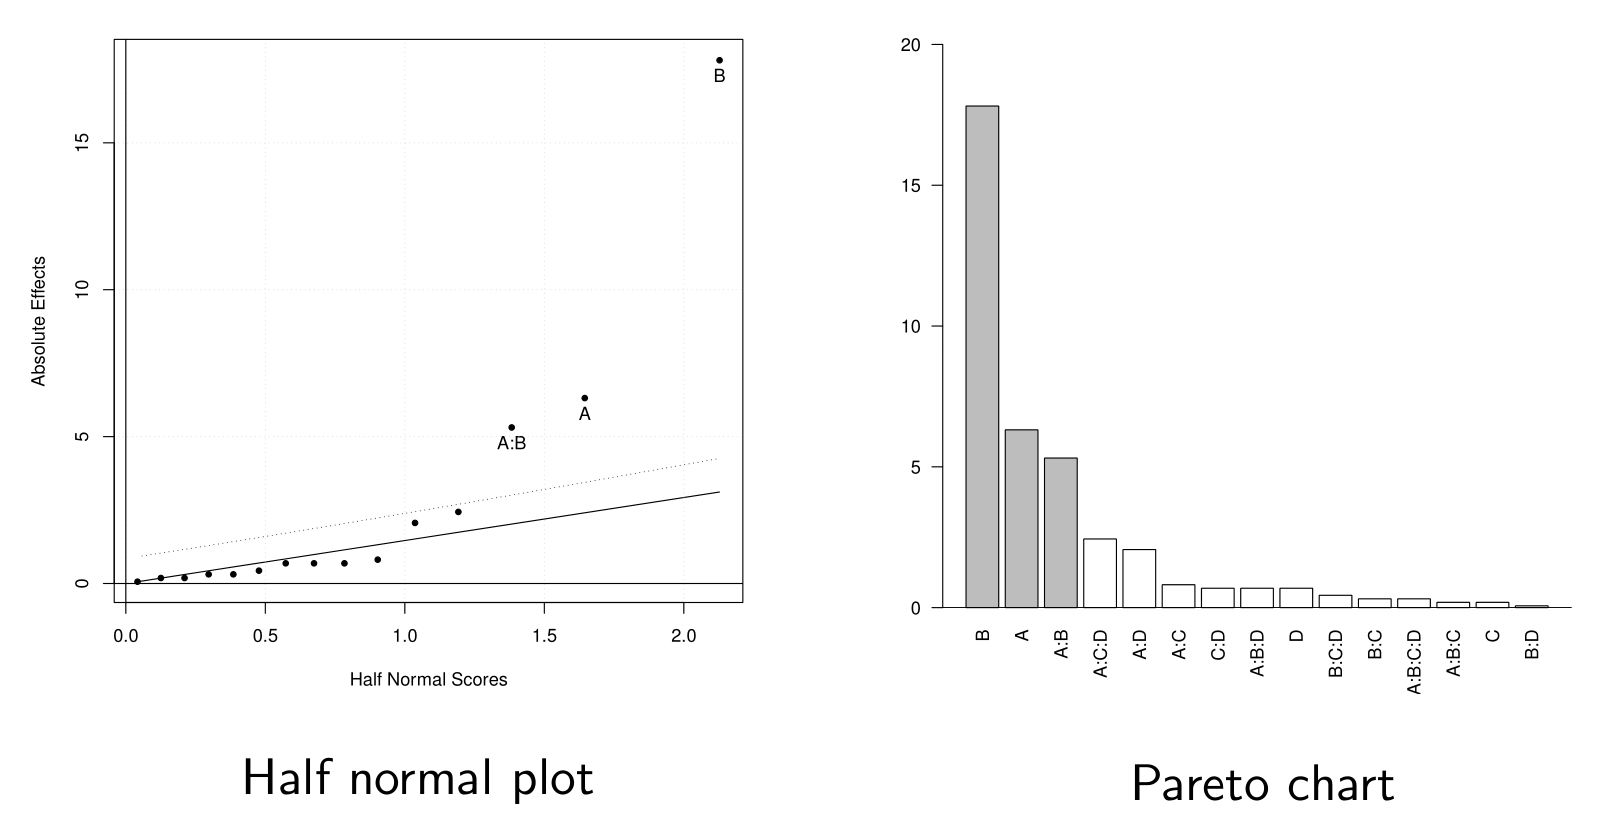
\includegraphics[width=0.8\linewidth]{img/significant_relevant_effects_factorial_design}
	\caption{Estimation of significant or relevant effects using Half-Normal plot and Pareto chart}
	\label{fig:significantrelevanteffectsfactorialdesign}
\end{figure}

\subsubsection{$2^k$ Fractional Factorial Design}
In the full factorial design the phenomena, that few major effects and few interaction effects are significant, can be observed. The idea is thus to combine higher order interactions with experimental error, which leads to a smaller model used to analyse the data.

\subsection{Response Surface Methodology}
The aim of this method is to optimise response which is influenced by several explanatory variables.
\begin{itemize}
	\item Detect important factors with a $2^k$ (fractional) factorial design
	\item Estimate main effects, determine direction of steepest ascent
	\item Find global optimum in the determined direction with a suitable design and additional experiments
\end{itemize}
This procedure is the response surface exploration based on a sequence of experimental designs.
\begin{equation*}
	E(y) = \eta = f(x_1, x_2)
\end{equation*}

\begin{figure}[tbh]
	\centering
	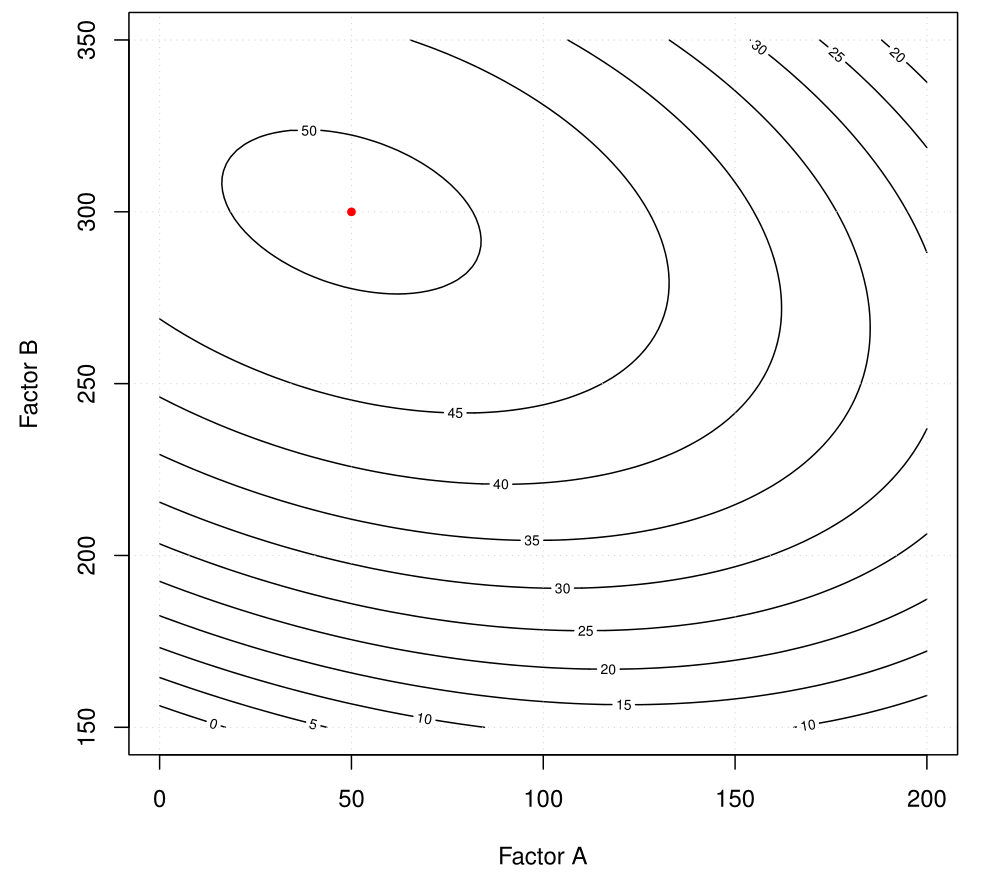
\includegraphics[width=0.6\linewidth]{img/contour_plot_second_order_response_surface}
	\caption{Contour plot of second-order response surface}
	\label{fig:contourplotsecondorderresponsesurface}
\end{figure}

The idea behind the response surface methodology is to find the optimal settings for the explanatory variables by experiment data. The response is a first- or second-order polynomial function for several variables, with the optimal fit for function $f$ being found analytically. This procedure is repeated until the optimum is reached.
\begin{equation*} 
	y=f(x_1,\dots,x_k) + \varepsilon \tag{fit response function}
\end{equation*}

\subsubsection{First-Order Design}
The initial settings of process variables are often far away from optimum. To tackle this problem, start with a first-order $2^k$ factorial design with additional measurements in the centre if the test conditions. Approximate the date with the linear model
\begin{equation*}
	y = \beta_0 + \beta_1 x_1 + \beta_2 x_2 + \dots + \beta_k x_k
\end{equation*}
of $k$ explanatory variables.

The advantage of this first order design is that the measurement error can be determined without assuming that the first-order linear model approximates the true response sufficiently well, and that the design can be used to detect deviations (curvature) from the first-order linear model.

\subsubsection{Statistical Test of Curvature in a $2^k$ Design}
\begin{itemize}[leftmargin=*,label=]
	\item \textbf{Hypothesis}
	\begin{itemize}
		\item $H_0$: no curvature in data
		\item $H_1$: curvature in the data
	\end{itemize}
	\item \textbf{Test statistic for curvature}
	\begin{equation*}
		t_{\text{curv}} = \frac{\samplemean{y}_c - \samplemean{y}_f}{\sqrt{s_c^2\left(\frac{1}{n_c} + \frac{1}{2^k}\right)}}
	\end{equation*}
	where $s_c^2$ is the variance of $n_c$ repetitions in the centre of the design.
\end{itemize}

Under the null hypothesis the test statistic $t_{\text{curv}}$ follows a $t$-distribution with $n_c-1$ degrees of freedom.

\subsubsection{Method of Steepest Ascent to find Optimum Setting}
Gradient of response function
\begin{align*}
	f(x_1, x_2) &= \beta_0 + \beta_1\cdot x_1 + \beta_2\cdot x_2\\
	\intertext{is}
	\nabla f(x_1, x_2) &= \begin{pmatrix}
		\frac{\partial}{\partial x_1}f(x_1, x_2)\\
		\frac{\partial}{\partial x_2}f(x_1, x_2)
	\end{pmatrix}\\
	&= \begin{pmatrix}
		\beta_1\\
		\beta_2
	\end{pmatrix}
\end{align*}
Estimated gradient points into the direction of the largest change, or maximal increase of the response, in the coded variable domain.

\subsubsection{Second-Order Response Surface with Interactions}
Second-order polynomials as surface function is used if there is curvature in the system or if the settings are close to the optimum making the response plane almost horizontal. Approximate the data with the linear model
\begin{equation*}
	y = \beta_0 + \sum_{i=1}^k\beta_i\cdot x_i + \sum_{i=1}^{k}\beta_{i,i}\cdot x_i^2 + \sum_{j=1}^k\sum_{i<j}^j\beta_{i,j}x_i x_j + \varepsilon
\end{equation*}
of $k$ explanatory variables, with its squares and all second-order interactions.

\subsubsection{Finding Optimum or Stationary Point}
To find the stationary point of the response function, set all $k$ partial derivatives equal to zero
\begin{align*}
	\frac{\partial}{\partial x_1}f(x_1,\dots,x_k) &= 0\\
	&\vdots\\
	\frac{\partial}{\partial x_k}f(x_1,\dots,x_k) &= 0\\
\end{align*}
and solve this system of $k$ linear equations for the $k$ unknowns $x_1,\dots,x_k$.

However, the solution could be a saddle point, which is more likely the more factors $k$ are involved. If the $k\times k$ Hessian matrix is positive definite for that solution $x_1,\dots,x_k$.
\begin{align*}
	\bm{H} f &= {\begin{bmatrix}{\dfrac {\partial ^{2}f}{\partial x_{1}^{2}}}&{\dfrac {\partial ^{2}f}{\partial x_{1}\,\partial x_{2}}}&\cdots &{\dfrac {\partial ^{2}f}{\partial x_{1}\,\partial x_{n}}}\\[2.2ex]{\dfrac {\partial ^{2}f}{\partial x_{2}\,\partial x_{1}}}&{\dfrac {\partial ^{2}f}{\partial x_{2}^{2}}}&\cdots &{\dfrac {\partial ^{2}f}{\partial x_{2}\,\partial x_{n}}}\\[2.2ex]\vdots &\vdots &\ddots &\vdots \\[2.2ex]{\dfrac {\partial ^{2}f}{\partial x_{n}\,\partial x_{1}}}&{\dfrac {\partial ^{2}f}{\partial x_{n}\,\partial x_{2}}}&\cdots &{\dfrac {\partial ^{2}f}{\partial x_{n}^{2}}}\end{bmatrix}} \tag{Hessian matrix of function $f$}\\
	x^T\bm{M}x &> 0 \forall x \tag{positive definiteness of matrix $\bm{M}$}
\end{align*}

\clearpage
\appendix
\section{Tables}
\begin{table}[H]
	\begin{tabularx}{\linewidth}{c | c c c | c c c | c c c | c}
		& \multicolumn{3}{c |}{$\samplemean{x}$ chart} & \multicolumn{3}{c |}{$R$ chart} & \multicolumn{3}{c |}{$s$ chart} & \\
		\hline
		$n$ & $A_1$ & $A_2$ & $A_3$ & $D_3$ & $D_4$ & $d_2$ & $B_3$ & $B_4$ & $c_4$ & $n$\\
		\hline
		$2$ & $3.760$ & $1.880$ & $2.659$ & $0.000$ & $3.267$ & $1.128$ & $0.000$ & $3.267$ & $0.7979$ & $2$ \\
		$3$ & $2.394$ & $1.023$ & $1.954$ & $0.000$ & $2.575$ & $1.693$ & $0.000$ & $2.568$ & $0.8862$ & $3$ \\
		$4$ & $1.880$ & $0.729$ & $1.628$ & $0.000$ & $2.282$ & $2.059$ & $0.000$ & $2.266$ & $0.9213$ & $4$ \\
		$5$ & $1.596$ & $0.577$ & $1.427$ & $0.000$ & $2.115$ & $2.326$ & $0.000$ & $2.089$ & $0.9400$ & $5$ \\
		$6$ & $1.410$ & $0.483$ & $1.287$ & $0.000$ & $2.004$ & $2.534$ & $0.030$ & $1.970$ & $0.9515$ & $6$ \\
		$7$ & $1.277$ & $0.419$ & $1.182$ & $0.076$ & $1.924$ & $2.704$ & $0.118$ & $1.882$ & $0.9594$ & $7$ \\
		$8$ & $1.175$ & $0.373$ & $1.099$ & $0.136$ & $1.864$ & $2.847$ & $0.185$ & $1.815$ & $0.9650$ & $8$ \\
		$9$ & $1.094$ & $0.337$ & $1.032$ & $0.184$ & $1.816$ & $2.970$ & $0.239$ & $1.761$ & $0.9693$ & $9$ \\
		$10$ & $1.028$ & $0.308$ & $0.975$ & $0.223$ & $1.777$ & $3.078$ & $0.284$ & $1.716$ & $0.9727$ & $10$ \\
		$11$ & $0.973$ & $0.285$ & $0.927$ & $0.256$ & $1.744$ & $3.173$ & $0.321$ & $1.679$ & $0.9754$ & $11$ \\
		$12$ & $0.925$ & $0.266$ & $0.886$ & $0.284$ & $1.716$ & $3.258$ & $0.354$ & $1.646$ & $0.9776$ & $12$ \\
		$13$ & $0.884$ & $0.249$ & $0.850$ & $0.308$ & $1.692$ & $3.336$ & $0.382$ & $1.618$ & $0.9794$ & $13$ \\
		$14$ & $0.848$ & $0.235$ & $0.817$ & $0.329$ & $1.671$ & $3.407$ & $0.406$ & $1.594$ & $0.9810$ & $14$ \\
		$15$ & $0.816$ & $0.223$ & $0.789$ & $0.348$ & $1.652$ & $3.472$ & $0.428$ & $1.572$ & $0.9823$ & $15$ \\
		$16$ & $0.788$ & $0.212$ & $0.763$ & $0.364$ & $1.636$ & $3.532$ & $0.448$ & $1.552$ & $0.9835$ & $16$ \\
		$17$ & $0.762$ & $0.203$ & $0.739$ & $0.379$ & $1.621$ & $3.588$ & $0.466$ & $1.534$ & $0.9845$ & $17$ \\
		$18$ & $0.738$ & $0.194$ & $0.718$ & $0.392$ & $1.608$ & $3.640$ & $0.482$ & $1.518$ & $0.9854$ & $18$ \\
		$19$ & $0.717$ & $0.187$ & $0.698$ & $0.404$ & $1.596$ & $3.689$ & $0.497$ & $1.503$ & $0.9862$ & $19$ \\
		$20$ & $0.697$ & $0.180$ & $0.680$ & $0.414$ & $1.586$ & $3.735$ & $0.510$ & $1.490$ & $0.9869$ & $20$ \\
		$21$ & $0.679$ & $0.173$ & $0.663$ & $0.425$ & $1.575$ & $3.778$ & $0.523$ & $1.477$ & $0.9876$ & $21$ \\
		$22$ & $0.662$ & $0.167$ & $0.647$ & $0.434$ & $1.566$ & $3.819$ & $0.534$ & $1.466$ & $0.9882$ & $22$ \\
		$23$ & $0.647$ & $0.162$ & $0.633$ & $0.443$ & $1.557$ & $3.858$ & $0.545$ & $1.455$ & $0.9887$ & $23$ \\
		$24$ & $0.632$ & $0.157$ & $0.619$ & $0.452$ & $1.548$ & $3.895$ & $0.555$ & $1.445$ & $0.9892$ & $24$ \\
		$25$ & $0.619$ & $0.153$ & $0.606$ & $0.459$ & $1.541$ & $3.931$ & $0.565$ & $1.435$ & $0.9896$ & $25$
	\end{tabularx}
	\caption{Factors for constructing control charts}
	\label{tbl:FactorsControlCharts}
\end{table}

\end{document}
